\documentclass{article}
\usepackage{emnlp2021}
\usepackage{times}
\usepackage{latexsym}
\usepackage[utf8]{inputenc}
\usepackage[T5]{fontenc}\usepackage{amsfonts}
\usepackage{microtype}
\usepackage{tabularx}
\usepackage{graphicx}
\usepackage{appendix}

\graphicspath{ {./images/} }

\title{DeepFake\\
Kĩ thuật chỉnh sửa ảnh khuôn mặt và phát hiện giả mạo}

\author{
Ruben Tolosana, Ruben Vera-Rodriguez, Julian Fierrez, Aythami Morales and Javier Ortega-Garcia\\
Đại học Autonoma Madrid, Tây Ban Nha
}
\begin{document}
\maketitle

\begin{abstract}

Khả năng truy cập tự do vào nguồn dữ liệu công khai trên internet, kết hợp những tiến bộ nhanh chóng của các kĩ thuật học sâu, đặc biệt là Generative Adversarial Networks (GAN), đã dẫn đến việc tạo ra nội dung đa phương tiện giả (nhưng có vẻ rất thật). Những nội dung giả này tác động nhiều mặt tiêu cực đối với xã hội hiện nay.

Bài báo này cung cấp một đánh giá kỹ lưỡng về các kĩ thuật chỉnh sửa trên ảnh khuôn mặt bao gồm phương pháp DeepFake và các phương pháp để phát hiện các chỉnh sửa đó. Có bốn loại chỉnh sửa trên khuôn mặt được nhắc đến trong bài này:
i) tổng hợp toàn bộ khuôn mặt,
ii) hoán đổi danh tính (DeepFakes),
iii) chỉnh sửa thuộc tính và
iv) hoán đổi biểu cảm.

Đối với mỗi nhóm chỉnh sửa, nhóm tác giả cung cấp thông tin chi tiết về (1) kĩ thuật chỉnh sửa - dữ liệu công khai hiện có và (2) các phương pháp chính để đánh giá công nghệ về các phương pháp phát hiện giả mạo. Trong số tất cả các khía cạnh được thảo luận trong bài báo này, nhóm tác giả đặc biệt chú ý đến thế hệ DeepFakes mới nhất, nêu bật những cải tiến và thách thức của nó đối với việc phát hiện giả mạo.

Ngoài thông tin khảo sát, nhóm tác giả cũng thảo luận về các vấn đề mở và xu hướng trong tương lai cần được xem xét trong lĩnh vực này.

\end{abstract}

\section{Giới thiệu} \label{sec:1-introduction}

Hình ảnh và video giả mạo bao gồm thông tin trên khuôn mặt được tạo ra bằng việc chỉnh sửa kĩ thuật số, đặc biệt là với phương pháp DeepFake \Citet{korshunov2018deepfakes}, đã trở thành một mối quan tâm lớn của công chúng gần đây. Thuật ngữ DeepFake phổ biến được dùng để chỉ một kĩ thuật dựa trên học sâu có thể tạo video giả bằng cách hoán đổi khuôn mặt của một người bằng khuôn mặt của người khác. Thuật ngữ này được bắt nguồn từ một người dùng Reddit có tên deepfakes cuối năm 2017, người dùng này đã phát triển một thuật toán học máy giúp anh ta chuyển khuôn mặt người nổi tiếng vào video khiêu dâm. Ngoài nội dung khiêu dâm giả mạo, một số cách sử dụng có hại hơn bao gồm tin tức giả, và những gian lận tài chính.
Nỗ lực nghiên cứu truyền thống trong pháp y để xây dựng nên tạo hình giờ đây đang chuyển sang nghiên cứu những chỉnh sửa trên khuôn mặt trong hình ảnh và video. Một phần của những thay đổi này được xây dựng dựa trên nghiên cứu trước đây về chống giả mạo sinh trắc học \Citet{cite13} \Citet{cite14} \Citet{cite15} và học sâu theo hướng dữ liệu hiện đại \Citet{cite16}, \Citet{dang2020detection}.

Mối quan tâm của cộng đồng ngày càng tăng về phát hiện khuôn mặt giả được thể hiện qua số lượng ngày càng tăng của các workshop trong các hội nghị hàng đầu, các dự án quốc tế như MediFor do Cơ quan Dự án Nghiên cứu Tiên tiến Bộ Quốc phòng Mỹ (DARPA) tài trợ, cũng như các cuộc thi như Forensics Challenge 1 (MFC2018 - Viện Tiêu chuẩn và Công nghệ Quốc gia Mỹ NIST) và Deepfake Detection Challenge 2 (DFDC - Facebook).

Theo truyền thống, số lượng và tính hiện thực của các chỉnh sửa trên khuôn mặt bị hạn chế do bị thiếu các công cụ chỉnh sửa phức tạp, yêu cầu chuyên môn về lĩnh vực cũng như quy trình phức tạp và tốn thời gian. Một sản phẩm giả mạo thời kì đầu được tạo để sửa đổi chuyển động môi của một người đang nói với một đoạn âm tthanh bằng cách tạo kết nối giữa âm thanh của đoạn âm thanh và hình dạng khuôn mặt của đối tượng. Tuy nhiên, từ đó cho đến nay, nhiều thứ đã phát triển nhanh chóng, hiện nay việc tự động tổng hợp các khuôn mặt không tồn tại hoặc chỉnh sửa khuôn mặt thật của một người trong hình ảnh/video ngày càng trở nên dễ dàng, nhờ: i) khả năng tiếp cận dữ liệu công khai quy mô lớn và ii) sự phát triển của các kĩ thuật học sâu loại bỏ nhiều bước chỉnh sửa thủ công, vd như Autoencoders (AE) và Generative Adversarial Networks (GAN) \Citet{kingma2013auto}, \Citet{goodfellow2014generative}. Một số các phần mềm miễn phí/mở và các ứng dụng di động như ZAO và FaceApp cho phép cho bất kỳ ai tạo ra các hình ảnh/video giả mạo mà không cần chút ít kinh nghiệm nào.

Để đối phó với những nội dung được làm giả một cách tinh vi, cộng đồng nghiên cứu đang nỗ lực để thiết kế các phương pháp để phát hiện chỉnh sửa trên khuôn mặt. Các phương pháp phát hiện giả mạo truyền thống trong kĩ thuật pháp y thường dựa trên: i) thông tin vân tay máy ảnh (in-camera fingerprint), định danh này do máy ảnh đưa vào thông tin cả phần cứng và phần mềm, chẳng hạn như ống kính được sử dụng \Citet{cite27}, bộ lọc màu \Citet{cite28}, \Citet{cite29}, kĩ thuật nén \Citet{cite30}, \Citet{cite31} và những thông tin tương tự. ii) thông tin định danh bên ngoài (out-camera fingerprint), các định danh bên ngoài được ghi vào bởi các phần mềm chỉnh sửa, chẳng hạn như copy-paste hoặc copy-move các phần tử khác nhau của hình ảnh \Citet{cite32}, \Citet{cite33}, giảm tốc độ khung hình trong video \Citet{cite34} \Citet{cite35} \Citet{cite36},… Tuy nhiên, hầu hết các đặc trưng được xem xét trong các phương pháp truyền thống phát hiện giả mảo phụ thuộc nhiều vào từng ảnh/video cụ thể, nên nó không đủ mạnh và linh hoạt để xử lý nguồn tin đa đạng hiện nay \Citet{cite6}, \Citet{cite8}, \Citet{cite16}. Mà điều này lại quan trọng đặc biệt trong cuộc sống hiện nay vì hầu hết nội dung giả mạo lan truyền trên các phương tiện như mạng xã hội, bản thân các nền tảng này đã tự động sửa đổi hình ảnh/video gốc bằng nhiều kĩ thuật như loại bỏ dữ liệu metadata, thay đổi độ nén và thay đổi kích thước \Citet{cite12}…

Bài báo này này cung cấp một đánh giá chuyên sâu về các kĩ thuật chỉnh sửa kĩ thuật số được áp dụng cho nội dung trên khuôn mặt. Cụ thể, nhóm tác giả đề cập đến bốn loại chỉnh sửa: i) tổng hợp toàn bộ khuôn mặt, ii) hoán đổi danh tính, iii) chỉnh sửa thuộc tính và iv) hoán đổi biểu hiện. Bốn kiểu chỉnh sửa khuôn mặt chính này đã được giới nghiên cứu xác lập rõ ràng, nhận được nhiều sự quan tâm nhất trong vài năm trở lại đây. Bên cạnh đó, nhóm tác giả cũng xem xét trong bài báo này này một số kĩ thuật chỉnh sửa khuôn mặt đầy thách thức và nguy hiểm khác chưa phổ biến như biến hình khuôn mặt (face morphing). Cuối cùng, để hoàn thiện, nhóm tác giả muốn nêu bật các bài báo khác gần đây trong lĩnh vực này. Trong \Citet{cite39}, các tác giả đề cập đến chủ đề DeepFake từ góc độ chung, đề xuất khuôn khổ R.E.A.L để quản lý rủi ro DeepFake.

Phần còn lại của bài báo được tổ chức như sau. Đầu tiên nhóm tác giả cung cấp trong phần II mô tả chung về các loại chỉnh sửa trên khuôn mặt. Sau đó, từ phần III đến phần VI, nhóm tác giả mô tả các khía cạnh chính của từng loại chỉnh sửa trên khuôn mặt bao gồm cơ sở dữ liệu công khai để nghiên cứu, phương pháp phát hiện và kết quả chuẩn. Phần VII tập trung vào các loại kĩ thuật chỉnh sửa khuôn mặt thú vị khác không được đề cập trong các phần trước. Cuối cùng, nhóm tác giả cung cấp trong phần VIII nhận xét kết luận của nhóm tác giả, nêu bật các vấn đề mở và xu hướng trong tương lai.


\section{PHÂN LOẠI CHỈNH SỬA KHUÔN MẶT} \label{sec:2-category}

Các kĩ thuật chỉnh sửa trên khuôn mặt có thể được phân loại thành bốn nhóm chính khác nhau về mức độ chỉnh sửa. Hình \ref{fig-1-category-and-example} tóm tắt từng nhóm chỉnh sửa trên khuôn mặt. Dưới đây là mô tả về từng loại trong số chúng, từ cấp độ chỉnh sửa cao hơn đến cấp độ thấp hơn:


\begin{figure*}[h!]
\caption{Phân loại chỉnh sửa trên khuôn mặt và ví dụ}
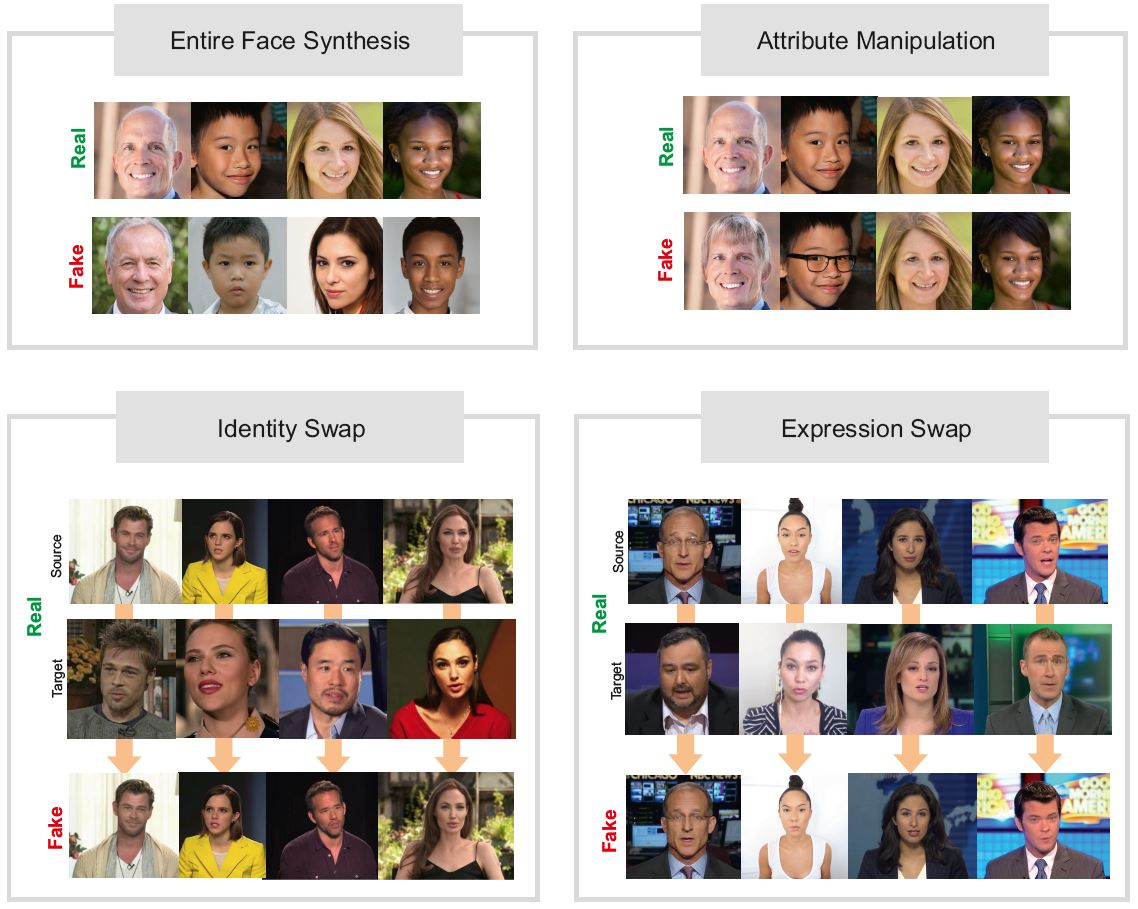
\includegraphics[width=\textwidth]{fig-1-category-and-example}
\label{fig-1-category-and-example}
\end{figure*}

\textbf{Tổng hợp toàn bộ khuôn mặt} (\textit{Entire Face Synthesis}): loại chỉnh sửa này tạo ra toàn bộ hình ảnh khuôn mặt không tồn tại, thường thông qua sức mạnh của GAN, ví dụ, thông qua cách tiếp cận StyleGAN gần đây đã đề xuất trong \Citet{karras2019style}. Những kĩ thuật này đạt được kết quả đáng kinh ngạc, tạo ra hình ảnh khuôn mặt chất lượng với độ chân thực cao. Hình 1 cho thấy một số ví dụ về tổng hợp toàn bộ khuôn mặt được tạo bằng StyleGAN. Kĩ thuật chỉnh sửa này có thể mang lại lợi ích cho nhiều lĩnh vực khác nhau như trò chơi điện tử, phim ảnh và các ngành công nghiệp mô hình 3D, nhưng nó cũng có thể được sử dụng cho các ứng dụng có hại như tạo hồ sơ giả rất giống thật trên mạng xã hội nhằm tạo ra thông tin sai lệch.

\textbf{Hoán đổi danh tính} (\textit{Attribute Manipulation}): kĩ thuật chỉnh sửa này bao gồm việc thay thế khuôn mặt của một người trong video bằng khuôn mặt của một người khác. Hai cách tiếp cận sau thường được xem xét: i) các kĩ thuật dựa trên đồ họa máy tính cổ điển như FaceSwap và ii) các kĩ thuật học sâu mới lạ được gọi là DeepFakes, ví dụ: ứng dụng di động ZAO gần đây. Các video rất thực về kiểu chỉnh sửa này rất nhiều trên Youtube hiện nay. Kiểu chỉnh sửa này có thể mang lại lợi ích cho nhiều lĩnh vực khác nhau, đặc biệt là ngành điện ảnh, ví dụ như trường hợp diễn viên Paul Walker gặp tai nạn trong khi vẫn còn cảnh quay ở phim Furious 7. Tuy nhiên, ở khía cạnh khác, nó cũng có thể được sử dụng cho các mục đích xấu như tạo video khiêu dâm giả của người nổi tiếng, gian lận tài chính, cùng nhiều mục đích khác.

\textbf{Chỉnh sửa thuộc tính} (\textit{Identity Swap}): kĩ thuật chỉnh sửa này, còn được gọi là face editing hoặc face retouching, bao gồm sửa đổi một số thuộc tính của khuôn mặt như màu tóc hoặc da, giới tính, tuổi, thêm kính, … \Citet{gonzalez2018facial}. Quá trình chỉnh sửa này thường được thực hiện thông qua GAN như cách tiếp cận StarGAN đã đề xuất trong \Citet{choi2018stargan}. Ví dụ cho kiểu chỉnh sửa này là ứng dụng trên di động phổ biến như FaceApp. Các nhà bán lẻ có thể sử dụng công nghệ này để người dùng được thử nhiều loại sản phẩm như mỹ phẩm và đồ trang điểm, kính hoặc kiểu tóc trong môi trường ảo.

\textbf{Hoán đổi biểu cảm} (\textit{Expression Swap}): chỉnh sửa này, còn được gọi là tái hiện khuôn mặt (face reenactment), bao gồm việc sửa đổi biểu cảm trên khuôn mặt của người. Mặc dù các kĩ thuật chỉnh sửa khác nhau đã đề xuất trong tài liệu, ví dụ như ở cấp độ hình ảnh thông qua các kiến trúc GAN phổ biến \Citet{liu2019stgan}, trong nhóm này nhóm tác giả tập trung vào 2 kĩ thuật phổ biến nhất Face2Face và NeuralTextures \Citet{thies2016face2face}, \Citet{thies2019deferred}, thay thế cho biểu cảm khuôn mặt của một người trong video với nét mặt của người khác. Kiểu thao túng này có thể được sử dụng với những hậu quả nghiêm trọng, ví dụ: video phổ biến về Mark Zuckerberg/Donald Trump nói những điều họ chưa từng nói

\section{TỔNG HỢP TOÀN BỘ KHUÔN MẶT} \label{sec:3-entire-face}

\subsection{Kĩ thuật chỉnh sửa và dữ liệu công khai} \label{sec:3-a-technique}

Kĩ thuật này tạo ra toàn bộ hình ảnh khuôn mặt không tồn tại. Bảng I tóm tắt các cơ sở dữ liệu công khai để nghiên cứu phát hiện các kĩ thuật chỉnh sửa hình ảnh dựa trên tổng hợp toàn bộ khuôn mặt. Bốn cơ sở dữ liệu khác nhau có liên quan ở đây, tất cả chúng đều dựa trên cùng một kiến trúc GAN: ProGAN \Citet{karras2017progressive} và StyleGAN \Citet{karras2019style}. Điều thú vị là mỗi hình ảnh giả mạo có thể được đặc trưng bởi một dấu vân tay GAN cụ thể giống như các hình ảnh tự nhiên được nhận dạng bằng dấu vân tay trên thiết bị (ví dụ PRNU). Trên thực tế, những dấu vân tay này dường như không chỉ phụ thuộc vào kiến trúc GAN mà còn phụ thuộc vào các instance khác nhau của nó \Citet{marra2019gans} \Citet{albright2019source} \Citet{jain2020detecting}.

\begin{figure}[h!]
\caption{Phân loại chỉnh sửa trên khuôn mặt và ví dụ}
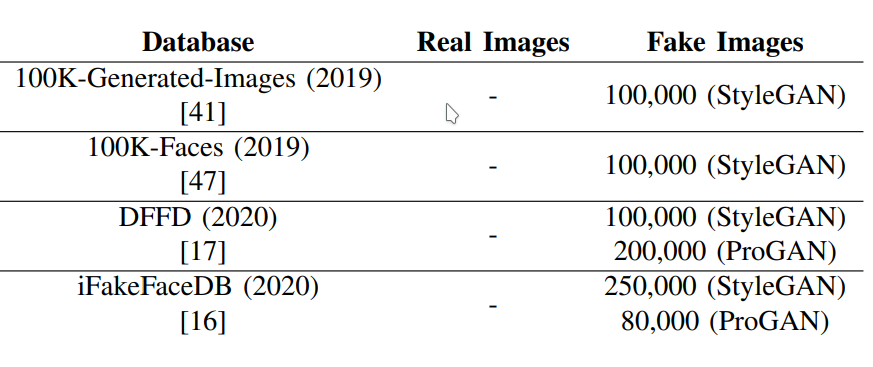
\includegraphics[width=\columnwidth]{table-1-database}
\label{table-1-database}
\end{figure}

Ngoài ra, như được chỉ ra trong Bảng I, điều quan trọng cần lưu ý là bốn cơ sở dữ liệu được đề cập chỉ chứa các hình ảnh giả được tạo ra bằng cách sử dụng các kiến trúc GAN. Để thực hiện các thí nghiệm phát hiện giả trên nhóm chỉnh sửa này, các nhà nghiên cứu cần thu được hình ảnh khuôn mặt thật từ các cơ sở dữ liệu công khai khác như CelebA \Citet{liu2015deep}, FFHQ \Citet{karras2019style}, CASIAWebFace \Citet{yi2014learning}, và VGGFace2 \Citet{cao2018vggface2}, trong số những cơ sở dữ liệu khác.

Các tác giả cung cấp mô tả bên cạnh mỗi cơ sở dữ liệu công khai. Trong \Citet{karras2019style}, Karras và cộng sự đã phát hành một tập dữ liệu 100.000 hình ảnh khuôn mặt tổng hợp, được đặt tên là \textbf{100K-Generated-Images}. Cơ sở dữ liệu này được tạo bằng cách sử dụng kiến trúc StyleGAN mà họ đề xuất, nó được huấn luyện bằng cách sử dụng bộ dữ liệu FFHQ \Citet{karras2019style}. StyleGAN là một phiên bản cải tiến của phương pháp tiếp cận phổ biến trước đây của họ là ProGAN. StyleGAN giới thiệu một phương pháp huấn luyện mới dựa trên việc cải thiện dần dần cả bộ sinh và bộ phân biệt. StyleGAN đề xuất một kiến trúc sinh thay thế dẫn đến sự phân tách tự động, không giám sát của các thuộc tính ở tầng cao (ví dụ: tư thế và nhận dạng khi được huấn luyện trên khuôn mặt người) và biến thể ngẫu nhiên trong các hình ảnh được tạo (ví dụ: tàn nhang, tóc) và nó cho phép kiểm soát tổng hợp trực quan, theo quy mô cụ thể.

Một cơ sở dữ liệu công khai khác là \textbf{100K-Faces}. Cơ sở dữ liệu này chứa 100.000 hình ảnh tổng hợp được tạo bằng StyleGAN. Trong cơ sở dữ liệu này, trái với cơ sở dữ liệu 100K-Generated-Images, mạng StyleGAN đã được huấn luyện bằng cách sử dụng khoảng 29.000 ảnh từ 69 kiểu khác nhau, xem xét ảnh khuôn mặt từ một kịch bản được điều khiển (ví dụ: với nền phẳng). Do đó, không có đồ vật kỳ lạ nào do StyleGAN tạo ra được đưa vào phần nền của hình ảnh.

Gần đây, Dang và cộng sự giới thiệu trong \Citet{dang2020detection} một cơ sở dữ liệu mới có tên \textbf{Diverse Fake Face Dataset} (Bộ dữ liệu đa dạng các khuôn mặt giả - DFFD). Các tác giả đã tạo ra 100.000 và 200.000 hình ảnh giả lần lượt thông qua các mô hình ProGAN và StyleGAN đã được huấn luyện trước.

\begin{figure}[h!]
\caption{Ví dụ ảnh fake và ảnh fake đã loại bỏ GAN fingerprint}
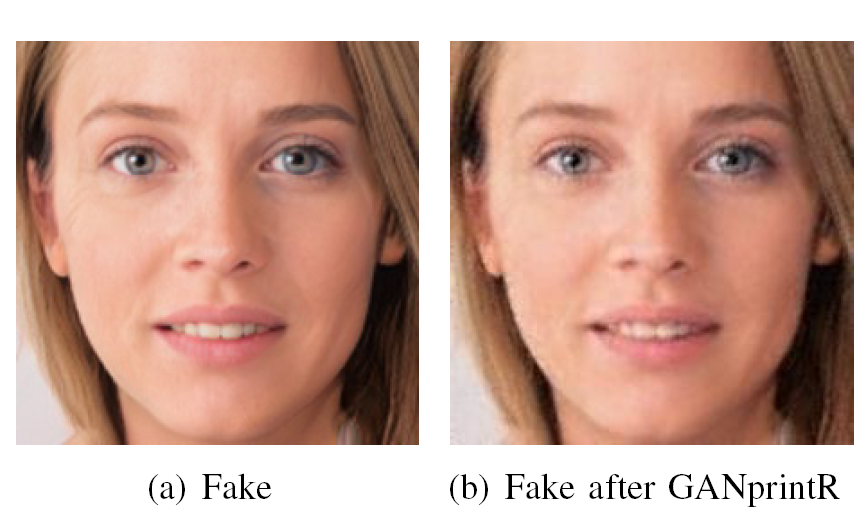
\includegraphics[width=\columnwidth]{fig-2-example}
\label{fig-2-example}
\end{figure}

Neves và cộng sự được trình bày trong \Citet{cite16} cơ sở dữ liệu \textbf{iFakeFaceDB}. Cơ sở dữ liệu này bao gồm 250.000 và 80.000 hình ảnh khuôn mặt tổng hợp được tạo tương ứng với StyleGAN và ProGAN. Một đặc trưng được bổ sung so với các cơ sở dữ liệu trước đây để làm khó việc phát hiện giả mạo, trong cơ sở dữ liệu này, các dấu vân tay do kiến trúc GAN tạo ra đã được loại bỏ thông qua một phương pháp có tên GANprintR (GAN fingerprint Removal - Loại bỏ dấu vân tay GAN), trong khi vẫn giữ được vẻ ngoài rất thực tế. Hình 2 cho thấy một ví dụ về hình ảnh giả được tạo trực tiếp bằng StyleGAN và phiên bản cải tiến của nó sau khi loại bỏ thông tin vân tay GAN. Kết quả của GANprintR, iFakeFaceDB gây ra nhiều thách thức hơn đối với các chương trình phát hiện giả mạo so với các cơ sở dữ liệu khác.

\subsection{Phát hiện chỉnh sửa} \label{sec:3-b-dectector}

Các nghiên cứu khác nhau gần đây đã đánh giá độ khó trong việc phát hiện xem khuôn mặt có phải là thật hay là khuôn mặt được sinh ra. Bảng II cho thấy sự so sánh của các cách tiếp cận phù hợp nhất trong lĩnh vực này. Đối với mỗi nghiên cứu, nhóm tác giả thêm vào thông tin liên quan đến phương pháp, bộ phân loại, hiệu suất tốt nhất và cơ sở dữ liệu được sử dụng. Các tác giả tô đậm kết quả tốt nhất đạt được cho mỗi cơ sở dữ liệu công khai. Điều quan trọng cần lưu ý là trong các nghiên cứu, tác giả sử dụng các phương pháp đánh giá kết quả khác nhau, ví dụ: Khu vực dưới đường cong (Area Under the Curve - AUC) hoặc Tỷ lệ lỗi ngang bằng (Equal Error Rate - EER), điều này gây khó cho việc so sánh kết quả các nghiên cứu.


\begin{figure*}[h!]
\caption{Bảng II: so sánh các phương pháp phát hiện chỉnh sửa}
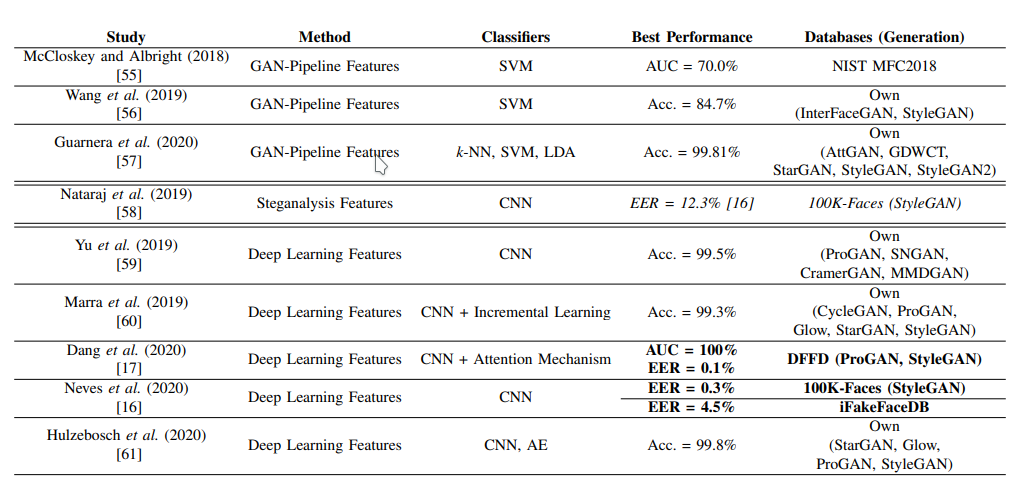
\includegraphics[width=\textwidth]{table-2-compare}
\label{table-2-compare}
\end{figure*}

Một số tác giả đề xuất phân tích pipeline bên trong GAN để phát hiện các hiện vật khác nhau giữa ảnh thật và ảnh giả. Trong \Citet{mccloskey2018detecting}, các tác giả đưa ra giả thuyết rằng màu sắc có sự khác biệt rõ rệt giữa hình ảnh thực và hình ảnh được tổng hợp. Họ đã đề xuất một hệ thống phát hiện dựa trên \textbf{các đặc điểm màu sắc và SVM} (support vector machine) để phân loại kết quả cuối cùng. Kết quả AUC cuối cùng là 70,0\% là hiệu suất tốt nhất khi đánh giá bằng tập dữ liệu NIST MFC2018 \Citet{guan2019mfc}

\Citet{wang1909fakespotter} phỏng đoán rằng theo dõi hành vi của neuron cũng có thể sử dụng như một công cụ phát hiện giả mạo vì các mẫu kích hoạt neuron từng lớp có thể nắm bắt các đặc trưng quan trọng hơn. Cách tiếp cận đã đề xuất của họ, được đặt tên là \textbf{FakeSpoter}, được trích xuất dưới dạng các đặc trưng của neuron thật và giả từ hệ thống nhận dạng khuôn mặt (ví dụ, VGG-Face \Citet{parkhi2015deep}, OpenFace \Citet{amos2016openface} và FaceNet \Citet{schroff2015facenet}), và sau đó huấn luyện một SVM cho bước phân loại cuối cùng. Các tác giả đã thử nghiệm bằng cách sử dụng khuôn mặt thật từ cơ sở dữ liệu CelebA-HQ \Citet{karras2017progressive} và FFHQ \Citet{karras2019style} và khuôn mặt tổng hợp được tạo thông qua InterFaceGAN \Citet{shen2020interpreting} và StyleGAN \Citet{karras2019style}, đạt được hiệu suất tốt nhất với độ chính xác 84,7\% bằng cách sử dụng mô hình FaceNet.

Các kết quả tốt hơn đã được báo cáo gần đây trong \Citet{guarnera2020deepfake}. Các tác giả đề xuất một hệ thống phát hiện giả mạo dựa trên việc phân tích \textbf{các dấu vết tích chập} (convolutional traces). Các đặc trưng được trích xuất bằng cách sử dụng thuật toán Maximum Expectation (Tối đa hóa kỳ vọng)) \Citet{moon1996expectation}. Các bộ phân loại phổ biến như k-Nearest Neighbors (k-NN), SVM và Linear Discriminant Analysis (LDA) đã được sử dụng cho bước cuối cùng. Phương pháp tiếp cận nà họ đề xuất đã được thử nghiệm bằng cách sử dụng các hình ảnh giả được tạo thông qua AttGAN \Citet{marra2019incremental}, GDWCT \Citet{cho2019image}, StarGAN \Citet{choi2018stargan}, StyleGAN và StyleGAN2 \Citet{karras2020analyzing}, đạt được độ chính xác 99,81\%.

Một số hệ thống phát hiện giả mạo lấy cảm hứng \textbf{từ phân tích mật mã} (steganalysis) cũng đã được xem xét. Nataraj và cộng sự đề xuất trong \Citet{nataraj2019detecting} một hệ thống phát hiện dựa trên sự kết hợp của ma trận đồng xuất hiện pixel và mạng tích chập (CNN). Cách tiếp cận này ban đầu đã được thử nghiệm thông qua cơ sở dữ liệu gồm các đối tượng và cảnh khác nhau được tạo thông qua CycleGAN \Citet{zhu2017unpaired}. Bên cạnh đó, các tác giả đã thực hiện một phân tích thú vị để xem hiệu quả của cách tiếp cận đã đề xuất khi chống lại các hình ảnh giả được tạo ra thông qua các kiến trúc GAN khác nhau (CycleGAN so với StarGAN), với kết quả nhìn chung là tốt. Phương pháp phát hiện này đã được triển khai sau đó trong \Citet{cite16} khi xem xét các hình ảnh từ cơ sở dữ liệu 100K-Faces, đạt được EER 12,3\% cho hiệu suất phát hiện ảnh giả tốt nhất.

Nhiều nghiên cứu cũng tập trung vào việc \textbf{phát hiện các dấu vân tay đặc biệt được chèn bởi các kiến trúc GAN} bằng phương pháp học sâu thuần túy. Yu và cộng sự đã đề xuất trong \Citet{yu2018attributing} một kiến trúc mạng phân bổ để ánh xạ hình ảnh đầu vào với hình ảnh dấu vân tay tương ứng của nó. Do đó, họ đã học được một dấu vân tay mô hình cho mỗi nguồn (mỗi loại GAN và ảnh thực), sao cho chỉ số tương quan giữa một dấu vân tay hình ảnh và mỗi dấu vân tay mô hình đóng vai trò như một phân loại logit softmax. Phương pháp của họ đã được thử nghiệm bằng cách sử dụng các khuôn mặt thật từ cơ sở dữ liệu CelebA \Citet{liu2015deep} và các khuôn mặt tổng hợp được tạo ra thông qua các phương pháp tiếp cận GAN khác nhau (ProGAN \Citet{karras2017progressive}, SNGAN \Citet{miyato2018spectral}, CramerGAN \Citet{bellemare2017cramer} và MMDGAN \Citet{binkowski2018demystifying}), đạt hiệu suất tốt nhất 99,5\%. Tuy nhiên, cách tiếp cận này dường như không hiệu quả lắm với cách gây nhiễu loạn hình ảnh đơn giản không nhìn thấy được như nhiễu, làm mờ, cắt xén hoặc nén, trừ khi các mô hình được huấn luyện lại một lần nữa.

Liên quan đến các điều kiện không nhìn thấy vừa nhận xét, Marra và cộng sự đã thực hiện trong \Citet{marra2019incremental} một nghiên cứu nhằm phát hiện các loại dữ liệu giả tạo chưa từng thấy. Cụ thể, họ đã đề xuất một phương pháp \textbf{phát hiện multi-task incremental learning} (học tăng dần đa tác vụ) để phát hiện và phân loại các loại hình ảnh được tạo từ những mẫu GAN mới, mà không làm giảm hiệu suất của các hình ảnh trước đó. Hai giải pháp khác nhau liên quan đến vị trí của bộ phân loại đã đã đề xuất dựa trên thuật toán iCaRL cho học tập tăng dần \Citet{rebuffi2017icarl}: i) Bộ phân loại nhiều tác vụ (MTMC) và ii) Bộ phân loại đơn nhiều tác vụ (MT-SC). Về khung thử nghiệm, năm phương pháp tiếp cận GAN khác nhau đã được xem xét trong nghiên cứu, CycleGAN \Citet{zhu2017unpaired}, ProGAN \Citet{karras2017progressive}, Glow \Citet{kingma2018glow}, StarGAN \Citet{choi2018stargan} và StyleGAN \Citet{karras2019style}. Cách tiếp cận của họ, dựa trên mô hình XceptionNet, đã đạt được kết quả đầy hứa hẹn là có thể phát hiện chính xác các hình ảnh được tạo ra bởi các thế hệ GAN khác nhau.

\textbf{Các cơ chế chú ý (attention)} cũng đã được áp dụng để cải thiện thêm quá trình huấn luyện của các hệ thống nhận diện. Dang và cộng sự thực hiện trong \Citet{dang2020detection} một phân tích đầy đủ về các loại chỉnh sửa trên khuôn mặt. Họ đề xuất sử dụng các cơ chế chú ý và các mô hình CNN phổ biến như XceptionNet và VGG16. Đối với toàn bộ chỉnh sửa tổng hợp khuôn mặt, các tác giả đã đạt được 100\% AUC cuối cùng và khoảng 0,1\% EER khi xem xét các khuôn mặt thật từ cơ sở dữ liệu CelebA \Citet{liu2015deep}, FFHQ \Citet{karras2019style} và FaceForensics ++ \Citet{cite12} và hình ảnh giả được tạo thông qua ProGAN \Citet{karras2017progressive} và StyleGAN \Citet{karras2019style}. Những kết quả ấn tượng đạt được cho thấy tầm quan trọng của các cơ chế chú ý \Citet{vaswani2017attention}.

Neves và cộng sự thực hiện trong \Citet{cite16} \textbf{thực nghiệm đánh giá chuyên sâu về khi xem xét các hệ thống phát hiện khác nhau với các điều kiện thử nghiệm khác nhau}, ví dụ các tình huống được kiểm soát và không kiểm soát. Bốn cơ sở dữ liệu giả mạo khác nhau đã được xem xét: i) 150.000 khuôn mặt giả được thu thập trực tuyến và dựa trên kiến trúc StyleGAN, ii) cơ sở dữ liệu công khai 100K khuôn mặt, iii) 80.000 khuôn mặt tổng hợp được tạo bằng ProGAN và iv) cơ sở dữ liệu iFakeFaceDB, phiên bản cải tiến của cơ sở dữ liệu giả mạo trong đó thông tin vân tay GAN đã bị xóa bằng cách sử dụng phương pháp GANprintR. Trong các kịch bản được kiểm soát, họ đã đạt được kết quả tương tự như các nghiên cứu tốt nhất trước đó (EER = 0,02\%). Tuy nhiên, trong các tình huống thử thách hơn, trong đó hình ảnh (thật và giả) đến từ các nguồn khác nhau (không khớp các bộ dữ liệu), hiệu suất phát hiện giả sẽ bị suy giảm cao. Cuối cùng, kết quả đạt được trên cơ sở dữ liệu iFakeFaceDB công khai của họ với EER = 4,5\% cho các trình phát hiện giả mạo tốt nhất cho thấy iFakeFaceDB khó như thế nào ngay cả đối với các phương pháp phát hiện tốt nhất. Liên quan đến nội dung giả tiên này, Cozzolino và cộng sự đã đề xuất trong \Citet{cozzolino2021spoc} một cách tiếp cận tương tự dựa trên GAN để đưa dấu vết camera vào hình ảnh tổng hợp nhằm đánh lừa các trình phát hiện giả tốt nhất.

Tương tự như \Citet{cite16}, Hulzebosch và cộng sự gần đây đã thực hiện \Citet{hulzebosch2020detecting} một phân tích chuyên sâu khi xem xét các tình huống khác nhau như mô hình chéo, dữ liệu chéo và xử lý hậu kỳ. Các phương pháp phát hiện giả dựa trên mạng Xception phổ biến và ForensicTransfer \Citet{cozzolino2018forensictransfer} - một phương pháp Autoencoder. Các kết quả nhìn chung không tốt thu được trong các kịch bản chưa từng quan sát (unseeen scenario), tương tự như \Citet{cite16}.

\section{ĐÁNH TRÁO DANH TÍNH}\label{sec:4-identity-swap}

\subsection{Kĩ thuật chỉnh sửa và Cơ sở dữ liệu công khai} \label{sec:4-a-technique}

Đây là một trong những hướng nghiên cứu phổ biến nhất hiện nay do mối quan tâm lớn của công chúng xung quanh DeepFakes. Nó bao gồm việc thay thế khuôn mặt của một người trong video bằng khuôn mặt của một người khác. Không giống như chỉnh sửa tổng hợp toàn bộ khuôn mặt - trong đó hình ảnh bị làm giả, trong hoán đổi danh tính, mục tiêu là tạo video giả.

Kể từ khi các cơ sở dữ liệu giả mạo công khai như cơ sở dữ liệu UADFV \Citet{li2018ictu}, cho đến cơ sở dữ liệu Celeb-DF và DFDC \Citet{li2020celeb}, \Citet{dolhansky2019deepfake} gần đây, nhiều cải tiến về hình ảnh đã được thực hiện, làm tăng tính chân thực của video giả. Kết quả là, cơ sở dữ liệu hoán đổi danh tính có thể được chia thành hai thế hệ khác nhau. Bảng III tóm tắt các chi tiết chính của từng cơ sở dữ liệu công khai, được nhóm lại theo từng thế hệ. Có thể thấy, trong kiểu chỉnh sửa trên khuôn mặt này, cả video thật và giả thường được đưa vào cơ sở dữ liệu.

\begin{figure}[h!]
\caption{Bảng III: Đánh tráo danh tính - Các cơ sở dữ liệu công khai}
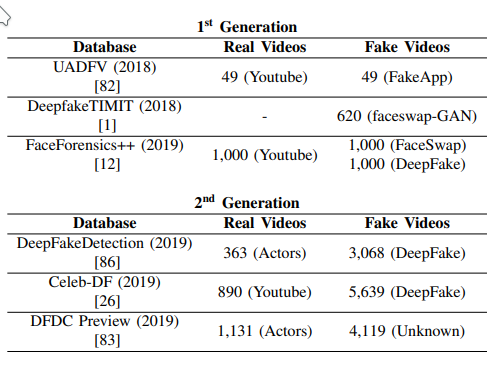
\includegraphics[width=\columnwidth]{table-3-database}
\label{table-3-database}
\end{figure}

Ba cơ sở dữ liệu khác nhau được nhóm vào thế hệ đầu tiên.

\textbf{UADFV} là một trong những cơ sở dữ liệu công khai đầu tiên \Citet{li2018ictu}. Cơ sở dữ liệu này bao gồm 49 video thật từ Youtube, được sử dụng để tạo 49 video giả thông qua ứng dụng di động FakeApp, hoán đổi tất cả khuôn mặt trong video gốc với khuôn mặt của Nicolas Cage. Do đó, chỉ có một danh tính được xem xét trong tất cả các video giả mạo. Mỗi video đại diện cho một cá nhân, với độ phân giải điển hình là 294x500 pixel và trung bình là 11,14 giây.

\Citet{korshunov2018deepfakes} đã giới thiệu cơ sở dữ liệu \textbf{Deepfake-TIMIT}. Cơ sở dữ liệu này bao gồm 620 video giả của 32 đối tượng từ cơ sở dữ liệu VidTIMIT \Citet{sanderson2009multi}. Video giả được tạo bằng thuật toán hoán đổi khuôn mặt dựa trên GAN. Theo cách tiếp cận này, mạng tổng hợp (genative network) được tiếp nối từ CycleGAN \Citet{zhu2017unpaired}, sử dụng trọng số của FaceNet \Citet{schroff2015facenet}. Phương pháp Multi-Task Cascaded Convolution Networks (mạng tích chập xếp tầng đa tác vụ) được sử dụng để việc phát hiện tốt hơn và căn chỉnh khuôn mặt \Citet{zhang2016joint}. Bên cạnh đó, bộ lọc Kalman cũng được coi là có tác dụng làm mịn các vị trí giới hạn biên (bounding box) trên các khung hình và loại bỏ hiện tượng rung trên mặt được hoán đổi. Trong DeepfakeTIMIT, hai chất lượng khác nhau được so sánh: i) chất lượng thấp (low quality - LQ) với hình ảnh 64x64 pixel và ii) chất lượng cao (high quality - HQ) với hình ảnh 128x128 pixel. Ngoài ra, các kĩ thuật pha trộn khác nhau đã được áp dụng cho các video giả mạo về mức chất lượng.

\begin{figure*}[h!]
\caption{Đánh tráo danh tính - Thế hệ thứ nhất}
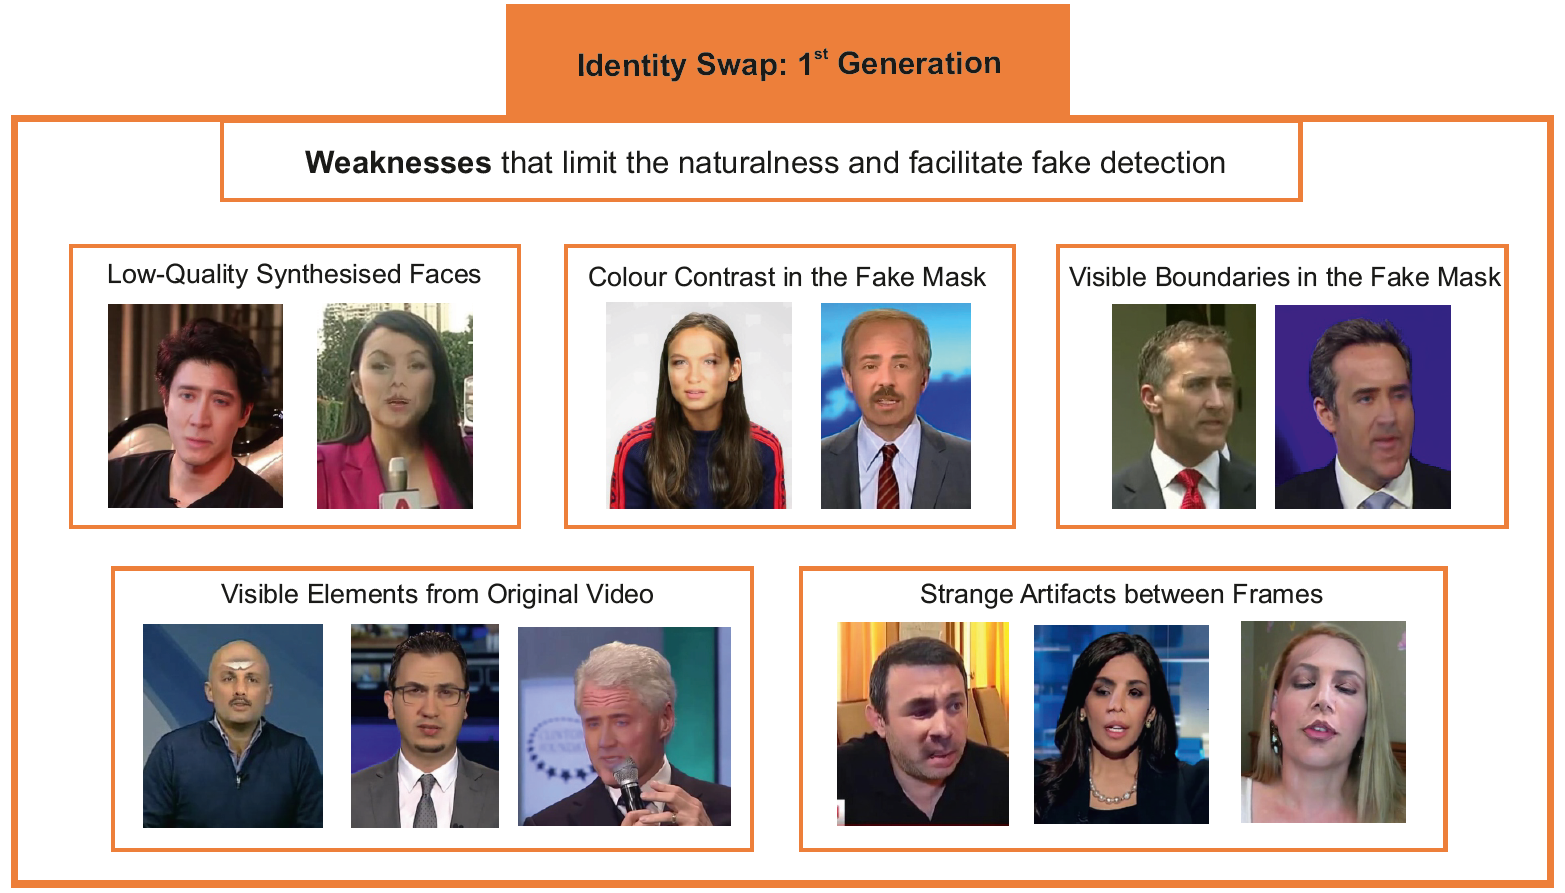
\includegraphics[width=\textwidth]{fig-3-id-swap-gen1}
\label{fig-3-id-swap-gen1}
\end{figure*}

Một trong những cơ sở dữ liệu phổ biến nhất về kiểu chỉnh sửa trên khuôn mặt này là \textbf{FaceForensics ++} \Citet{cite12}. Cơ sở dữ liệu này được giới thiệu vào đầu năm 2019 như một phần mở rộng của cơ sở dữ liệu FaceForensics ban đầu \Citet{rossler2018faceforensics}, chỉ tập trung vào hoán đổi biểu cảm. FaceForensics ++ chứa 1000 video thực được trích xuất từ Youtube. Về các video giả hoán đổi danh tính, chúng được tạo bằng cách sử dụng cả đồ họa máy tính và phương pháp DeepFake (ví dụ learning approach). Đối với phương pháp đồ họa máy tính, các tác giả đã xem xét thuật toán FaceSwap có sẵn công khai, trong khi đối với phương pháp DeepFake, các video giả được tạo thông qua triển khai DeepFake FaceSwap trên GitHub. Phương pháp hoán đổi khuôn mặt bao gồm căn chỉnh khuôn mặt, tối ưu hóa Gauss Newton và kết hợp hình ảnh để hoán đổi khuôn mặt của người gốc sang người mục tiêu. Phương pháp DeepFake, như được chỉ ra trong \Citet{cite12}, dựa trên hai bộ autoencoder với một bộ mã hóa dùng chung được huấn luyện để tạo lại hình ảnh huấn luyện của khuôn mặt ban đầu và mặt mục tiêu tương ứng. Bộ phát hiện khuôn mặt được sử dụng để cắt và căn chỉnh hình ảnh. Để tạo ra một hình ảnh giả, bộ mã hóa encoder và bộ giải mã decover (đã được huấn luyện) được áp dụng cho mặt đích. AutoEncoder output sau đó được trộn với phần còn lại của hình ảnh bằng cách sử dụng chương trình Poisson image editing \Citet{perez2003poisson}. Về số liệu của cơ sở dữ liệu FaceForensics ++, 1000 video giả đã được tạo cho mỗi cách tiếp cận. Sau đó, một tập dữ liệu mới có tên \textbf{DeepFakeDetection}, được nhóm bên trong thế hệ thứ 2 do tính hiện thực cao hơn, đã được đưa vào khuôn khổ FaceForensics ++ với sự hỗ trợ của Google \Citet{dufour2019contributing}. Tập dữ liệu này bao gồm 363 video thực từ 28 diễn viên được trả tiền trong 16 cảnh khác nhau. Ngoài ra, 3068 video giả mạo được đưa vào tập dữ liệu dựa trên việc triển khai DeepFake FaceSwap GitHub. Điều quan trọng cần lưu ý là đối với cả cơ sở dữ liệu FaceForensics ++ và DeepFakeDetection, các mức chất lượng video khác nhau được xem xét, cụ thể: i) RAW (chất lượng gốc), ii) HQ (tham số lượng tử hóa tốc độ không đổi bằng 23) và iii) LQ (không đổi tham số lượng tử hóa tỷ lệ bằng 40). Khía cạnh này mô phỏng các kĩ thuật xử lý video thường được áp dụng trong mạng xã hội.

Về các cơ sở dữ liệu được bao gồm trong thế hệ thứ 2, nhóm tác giả nhấn mạnh các cơ sở dữ liệu \textbf{Celeb-DF} và \textbf{DFDC }gần đây được phát hành vào cuối năm 2019. Li và cộng sự đã trình bày trong \Citet{li2020celeb} cơ sở dữ liệu CelebDF. Cơ sở dữ liệu này nhằm mục đích cung cấp các video giả có chất lượng hình ảnh tốt hơn, tương tự như các video phổ biến được chia sẻ trên Internet, so với các cơ sở dữ liệu trước đây có chất lượng hình ảnh thấp với nhiều hiện vật có thể nhìn thấy được. Celeb-DF bao gồm 890 video thực được trích xuất từ Youtube và 5.639 video giả, được tạo thông qua phiên bản tinh chỉnh của thuật toán tạo DeepFake công khai, cải thiện các khía cạnh như độ phân giải thấp của các khuôn mặt tổng hợp và sự không nhất quán về màu sắc.

Facebook phối hợp với các công ty và tổ chức học thuật khác như Microsoft, Amazon và MIT đã đưa ra vào cuối năm 2019 một thử thách mới có tên là \textbf{Deepfake Detection Challenge} (DFDC) \Citet{dolhansky2019deepfake}. Đầu tiên, họ phát hành tập dữ liệu xem trước bao gồm 1.131 video thật từ 66 diễn viên trả phí và 4.119 video giả. Các video giả được tạo bằng hai cách tiếp cận khác nhau không xác định. Tập dữ liệu DFDC hoàn chỉnh đã được phát hành sau đó và bao gồm hơn 470 GB nội dung (thật và giả).

\begin{figure*}[h!]
\caption{Đánh tráo danh tính - Thế hệ thứ hai}
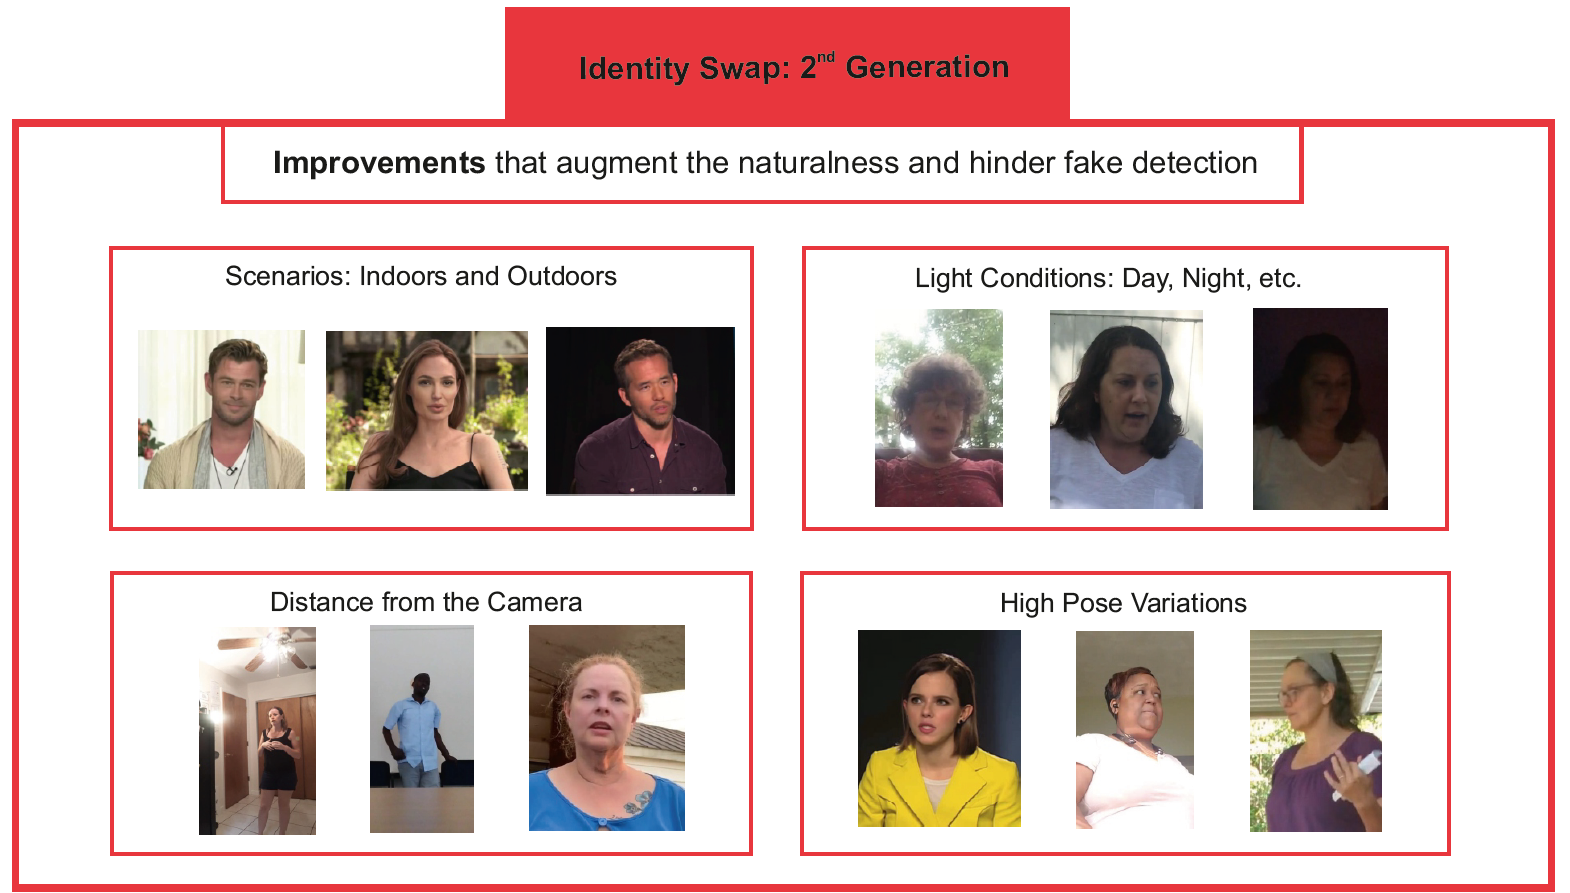
\includegraphics[width=\textwidth]{fig-4-id-swap-gen2}
\label{fig-4-id-swap-gen2}
\end{figure*}

Nhìn chung, video giả từ thế hệ thứ nhất có đặc điểm: i) khuôn mặt tổng hợp chất lượng thấp, ii) độ tương phản màu khác nhau giữa khuôn mặt giả và da của khuôn mặt gốc, iii) ranh giới nhìn thấy được của mặt nạ giả, iv) các yếu tố trên khuôn mặt có thể nhìn thấy từ video gốc, v) các biến thể tư thế thấp và vi) tạo tác kỳ lạ giữa các khung hình liên tiếp. Ngoài ra, họ thường xem xét các kịch bản được kiểm soát về vị trí máy ảnh và điều kiện ánh sáng. Nhiều khía cạnh trong số này đã được cải thiện thành công trong cơ sở dữ liệu của thế hệ thứ 2, không chỉ ở cấp độ trực quan mà còn về khả năng thay đổi (các kịch bản trong tự nhiên). Ví dụ: cơ sở dữ liệu DFDC gần đây xem xét các tình huống thu nhận khác nhau (nghĩa là trong nhà và ngoài trời), điều kiện ánh sáng (ví dụ ngày, đêm, …), khoảng cách từ người đến máy ảnh và các biến thể tư thế, trong số những người khác. Hình 3 tóm tắt bằng đồ thị những điểm yếu có trong cơ sở dữ liệu hoán đổi danh tính của thế hệ thứ nhất và những cải tiến được thực hiện trong thế hệ thứ hai. Cuối cùng, cũng rất thú vị khi nhận xét rằng số lượng lớn hơn các video giả mạo được đưa vào cơ sở dữ liệu của thế hệ thứ 2.

\subsection{Phát hiện chỉnh sửa} \label{sec:4-b-detector}

Sự phát triển của các phương pháp mới để phát hiện các chỉnh sửa hoán đổi danh tính liên tục phát triển. Bảng IV cung cấp sự so sánh các phương pháp phát hiện phù hợp nhất trong lĩnh vực này. Đối với mỗi nghiên cứu, nhóm tác giả bao gồm thông tin liên quan đến phương pháp, bộ phân loại, hiệu suất tốt nhất và cơ sở dữ liệu cho nghiên cứu. Các tác giả tô đậm kết quả tốt nhất đạt được cho mỗi cơ sở dữ liệu công khai. Điều quan trọng cần lưu ý là trong các nghiên cứu, có một số các cách đánh giá kết quả khác nhau được sử dụng (ví dụ, AUC và EER), điều này gây phức tạp việc so sánh giữa các nghiên cứu. Những kết quả này đã được trích xuất từ \Citet{li2020celeb} và không có trong các ấn phẩm gốc.

% bảng 4 quá dài để đưa vào

Các nghiên cứu đầu tiên trong lĩnh vực này tập trung vào các tác phẩm nghe nhìn (audio-visual) tồn tại trong thế hệ video giả đầu tiên. Korshunov và Marcel đã đánh giá \Citet{korshunov2018deepfakes} phương pháp tiếp cận cơ bản (baseline approaches) dựa trên sự không nhất quán giữa chuyển động môi và âm thanh phát ra, cũng như một số đặc trưng của hệ thống dựa trên hình ảnh thường được sử dụng trong sinh trắc học. Đối với trường hợp đầu tiên, họ coi hệ số tương quan Mel-Frequency Cepstral (Mel-Frequency Cepstral Coefficients - MFCC) là đặc trưng âm thanh và khoảng cách giữa các mốc miệng là đặc trưng hình ảnh. Phân tích thành phần chính (Principal Component Analysis - PCA) sau đó được sử dụng để giảm kích thước của các block đặc trưng và cuối cùng là Recurrent Neural Networks (RNNs) dựa trên Long Short-Term Memory (LSTM) để phát hiện video giả (dựa trên \Citep{korshunov2018speaker}). Đối với trường hợp thứ hai, họ đánh giá các phương pháp phát hiện dựa trên: i) các khuôn mặt thô làm đặc trưng, và ii) các thước đo chất lượng hình ảnh (IQM) \Citep{galbally2013image}. Đặc biệt, họ đã sử dụng một bộ 129 đặc trưng liên quan đến các phép đo như tỷ lệ tín hiệu trên nhiễu, độ rõ nét, độ mờ, … PCA với LDA hoặc SVM dùng để phân loại. Phương pháp phát hiện đã đề xuất của họ dựa trên IQM + SVM đã cung cấp kết quả tốt nhất, với EER cuối cùng là 3,3\% và 8,9\% cho các kịch bản LQ và HQ của cơ sở dữ liệu DeepfakeTIMIT tương ứng.

Trong nhánh này, Matern và cộng sự đã đề xuất trong \Citet{matern2019exploiting} hệ thống phát hiện giả mạo \textbf{dựa trên các khía cạnh thị giác} tương đối đơn giản như màu mắt, phản xạ bị thiếu và các chi tiết bị thiếu trong vùng mắt và răng. Hai bộ phân loại khác nhau đã được xem xét trong phân tích này: i) một mô hình hồi quy logistic và ii) perceptron nhiều lớp (Multi Layer Perceptron - MLP) \Citep{goodfellow2016deep}. Phương pháp tiếp cận của họ đã được thử nghiệm bằng cách sử dụng cơ sở dữ liệu riêng, đạt được 85,1\% AUC cho hệ thống MLP.

Hệ thống phát hiện giả \textbf{dựa trên nét mặt và chuyển động của đầu} cũng đã đã đề xuất trong tài liệu. Yang và cộng sự \Citet{yang2019exposing} quan sát thấy rằng một số DeepFakes được tạo ra bằng cách ghép các vùng khuôn mặt tổng hợp vào hình ảnh gốc và làm như vậy, đưa ra các lỗi có thể được phát hiện khi ước tính tư thế đầu 3D từ hình ảnh khuôn mặt. Do đó, họ đã thực hiện một nghiên cứu dựa trên sự khác biệt giữa các tư thế đầu được tính bằng cách sử dụng một bộ đầy đủ các điểm mốc trên khuôn mặt (68 trích từ DLib \Citep{king2009dlib}) và các điểm ở vùng trung tâm khuôn mặt để phân biệt DeepFakes với video thực. Sau khi các đặc trưng này được trích xuất và chuẩn hóa (trung bình và độ lệch chuẩn), SVM sử dụng để phân loại. Cách tiếp cận của họ được đánh giá ban đầu với cơ sở dữ liệu UADFV, đạt được 89,0\% AUC. Tuy nhiên, mô hình được huấn luyện trước này (sử dụng cơ sở dữ liệu UADFV) dường như không khái quát hóa tốt cho các cơ sở dữ liệu khác như được mô tả trong Bảng IV.

\begin{figure*}[h!]
\caption{Bảng IV: So sánh các cách phát hiện}
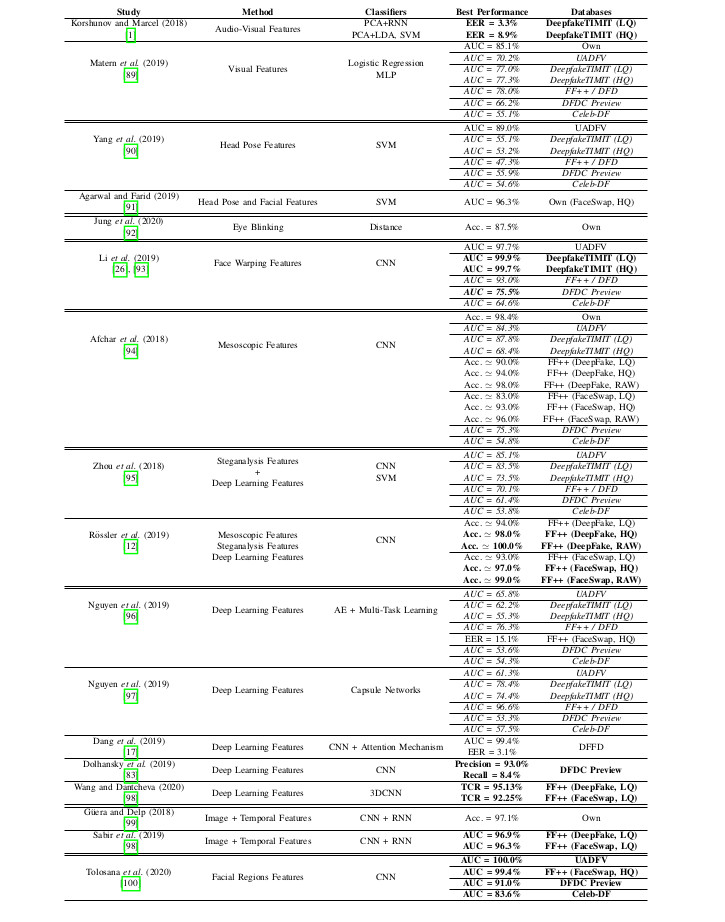
\includegraphics[width=\textwidth]{table-4-compare}
\label{table-4-compare}
\end{figure*}

Agarwal và Farid trong \Citet{agarwal2019protecting} đề xuất một hệ thống phát hiện \textbf{dựa trên cả nét mặt và chuyển động của đầu}. Đối với việc trích xuất đặc trưng, bộ công cụ OpenFace2 đã được sử dụng \Citep{baltrusaitis2018openface}, thu được cường độ và sự xuất hiện cho 18 đơn vị hành động trên khuôn mặt khác nhau liên quan đến các chuyển động của cơ mặt như nâng má, nhăn mũi, căng miệng, … Ngoài ra, bốn đặc trưng liên quan đến các chuyển động của đầu đã được xét. Do đó, mỗi video clip dài 10 giây được giảm xuống một vectơ đặc trưng có kích thước 190 bằng cách sử dụng tương quan Pearson để đo mức độ tuyến tính giữa các đối tượng địa lý. Cuối cùng, các tác giả đã xem xét một SVM để phân loại. Về khuôn khổ thử nghiệm, các tác giả đã xây dựng cơ sở dữ liệu của riêng họ dựa trên các video tải xuống từ YouTube về những người quan tâm đang nói chuyện trong bối cảnh trang trọng, ví dụ: địa chỉ hàng tuần, phỏng vấn tin tức và bài phát biểu trước công chúng. Trong hầu hết các video, người đó chủ yếu quay mặt về phía máy ảnh. Về các video DeepFake, các tác giả đã huấn luyện một GAN cho mỗi người dựa trên facewap-GAN. Cách tiếp cận của họ đã đạt được kết quả tốt nhất là 96,3\% AUC, đủ linh hoạt trước các ngữ cảnh và kĩ thuật chỉnh sửa mới.

\textbf{Nháy mắt} \Citep{daza2020mebal} cũng đã được nghiên cứu để phát hiện video giả. Trong \Citet{jung2020deepvision}, các tác giả đề xuất một thuật toán gọi là DeepVision để phân tích những thay đổi trong các kiểu nhấp nháy. Phương pháp tiếp cận của họ dựa trên sự kết hợp của Fast-HyperFace \Citep{ranjan2017hyperface} và Eye-Aspect-Ratio (EAR) \Citep{soukupova2016eye} để phát hiện khuôn mặt và thu được tỷ lệ khung hình của mắt. Cuối cùng, các đặc trưng dựa trên số lần nhấp nháy và khoảng thời gian đã được trích xuất để quyết định video là thật hay giả. Cách tiếp cận này đạt được độ chính xác cuối cùng là 87,5\% so với cơ sở dữ liệu riêng tư.

Một nhánh nghiên cứu nữa dựa trên việc \textbf{phát hiện các đối tượng (artifact)} được đưa vào bởi pipeline chỉnh sửa trên khuôn mặt. Trong \Citet{li2018exposing}, Li và Lyu đưa ra giả thuyết rằng một số thuật toán DeepFake chỉ có thể tạo ra những hình ảnh có độ phân giải hạn chế, những hình ảnh này cần được làm mịn thêm để khớp với khuôn mặt ban đầu trong video nguồn. Những chuyển đổi như vậy để lại các artifact đặc biệt trong các video DeepFake thu được. Do đó, các tác giả đã đề xuất một hệ thống phát hiện dựa trên CNN để phát hiện sự hiện diện của các artifact đó từ các vùng khuôn mặt được phát hiện và các khu vực xung quanh. Bốn mô hình CNN khác nhau được huấn luyện từ đầu: VGG16 \Citep{simonyan2014very}, ResNet50, ResNet101 và ResNet152 \Citep{he2016deep}. Phương pháp phát hiện đề xuất của họ đã được thử nghiệm bằng cách sử dụng cơ sở dữ liệu UADFV và DeepfakeTIMIT, vượt trội hơn so với kết quả tốt nhất trên cơ sở dữ liệu được xét.

Li và cộng sự đã đề xuất sau đó trong \Citet{li2020celeb} một phiên bản cải tiến của công việc được trình bày trong \Citet{li2018exposing}. Trong trường hợp này, các tác giả đã đưa vào một module gộp kim tự tháp không gian (spatial pyramid) mới để xử lý tốt hơn các biến thể trong độ phân giải \Citep{he2015spatial}. Phương pháp phát hiện này được đánh giá bằng cách sử dụng các cơ sở dữ liệu khác nhau, đạt được kết quả tốt nhất trong một số cơ sở dữ liệu.

Các phương pháp tiếp cận dựa trên các đặc trưng của code (steganalysis - phân tích mật mã) cũng đã đã đề xuất trong tài liệu. Afchar và cộng sự đã đề xuất trong \Citet{afchar2018mesonet} hai mạng khác nhau bao gồm ít lớp để tập trung vào các đặc tính trung mô của hình ảnh: i) một mạng CNN bao gồm 4 lớp chập, tiếp theo là một lớp được kết nối đầy đủ (Meso-4), và ii) một sửa đổi của Meso-4 bao gồm một biến thể của module Inception được giới thiệu trong \Citep{szegedy2015going}, được đặt tên là \textbf{MesoInception-4}. Cách tiếp cận đã đề xuất của họ ban đầu được thử nghiệm với DeepFakes bằng cách sử dụng cơ sở dữ liệu riêng, đạt được 98,4\% độ chính xác. Mô hình phát hiện được huấn luyện trước đó đã được thử nghiệm dựa trên các cơ sở dữ liệu chưa từng gặp trong \Citet{li2020celeb}, được chứng minh là một phương pháp mạnh mẽ trong một số trường hợp như với FaceForensics ++.

Zhou và cộng sự đã đề xuất một \textbf{mạng hai luồng để phát hiện chỉnh sửa trên khuôn mặt}. Đặc biệt, các tác giả đã xem xét sự kết hợp của hai luồng: i) luồng phân loại khuôn mặt dựa trên CNN GoogLeNet \Citep{szegedy2015going} để phát hiện xem hình ảnh khuôn mặt có phải là giả mạo hay không và ii) luồng bộ ba đường dẫn được huấn luyện bằng cách sử dụng các đặc trưng phân tích ẩn các bản vá hình ảnh bị mất bộ ba và SVM để phân loại. Hệ thống ban đầu được huấn luyện để phát hiện các chỉnh sửa hoán đổi biểu cảm. Tuy nhiên, Li và cộng sự được đánh giá trong \Citet{li2020celeb} khả năng tổng quát hóa của mô hình được huấn luyện trước (được huấn luyện bằng ứng dụng SwapMe) để phát hiện các chỉnh sửa hoán đổi danh tính, dẫn đến trở thành một trong những cách tiếp cận mạnh nhất đối với cơ sở dữ liệu Celeb-DF \Citet{li2020celeb}.

Rossler và cộng sự đã tiến hành \textbf{phân tích toàn diện các phương pháp phát hiện giả} khác nhau. sử dụng cơ sở dữ liệu FaceForensics ++ \Citet{cite12}. Năm hệ thống phát hiện khác nhau đã được đánh giá: i) hệ thống dựa trên CNN được huấn luyện thông qua các đặc trưng phân tích mật thủ công \Citep{cozzolino2017recasting}, ii) hệ thống dựa trên CNN có các lớp tích chập được thiết kế đặc biệt để loại bỏ nội dung cấp cao của hình ảnh \Citep{bayar2016deep}, iii) hệ thống dựa trên CNN với lớp tổng hợp toàn cầu tính toán bốn thống kê (trung bình, phương sai, tối đa và tối thiểu) \Citep{rahmouni2017distinguishing}, iv) hệ thống phát hiện CNN MesoInception-4 được mô tả trong \Citet{afchar2018mesonet}, và cuối cùng là v) Hệ thống dựa trên CNN XceptionNet \Citep{chollet2017xception} được huấn luyện trước bằng cách sử dụng cơ sở dữ liệu ImageNet \Citep{deng2009imagenetxception} và được huấn luyện lại cho nhiệm vụ phát hiện chỉnh sửa trên khuôn mặt. Nhìn chung, hệ thống phát hiện dựa trên kiến trúc\textbf{ XceptionNet đã cung cấp kết quả tốt nhất} trong cả hai loại phương pháp chỉnh sửa, DeepFakes và FaceSwap. Ngoài ra, các hệ thống phát hiện đã được đánh giá xem xét các mức chất lượng video khác nhau để mô phỏng quá trình xử lý video của nhiều mạng xã hội. Trong tình huống thực này, độ chính xác của tất cả các hệ thống phát hiện đều giảm khi giảm chất lượng video, cho thấy rằng nhiệm vụ này trong các tình huống thực tế là rất khó khăn.

Nguyen và cộng sự \Citet{nguyen2019multi} đã đề xuất một \textbf{hệ thống CNN sử dụng đặc trưng học tập đa tác vụ (multi-task learning)} để đồng thời phát hiện các video giả mạo và xác định vị trí các khu vực bị thao túng. Họ coi là một hệ thống phát hiện dựa trên một autoencoder. Cụ thể, họ đề xuất sử dụng bộ giải mã hình chữ Y để chia sẻ thông tin có giá trị giữa các nhiệm vụ phân loại, phân đoạn và tái thiết, cải thiện hiệu suất tổng thể bằng cách giảm mất mát. Phương pháp tiếp cận đề xuất của họ được đánh giá với phương pháp chỉnh sửa FaceSwap cho cơ sở dữ liệu FaceForensics ++ \Citet{rossler2018faceforensics}, đạt được hiệu suất tốt nhất là 15,07\% EER, khác xa so với các phương pháp phát hiện khác. Ngoài ra, mô hình này dường như không khái quát hóa tốt cho các cơ sở dữ liệu khác, với kết quả dưới 80\% AUC.

Sau đó, các tác giả đã trình bày trong \Citet{nguyen2019use} một hệ thống phát hiện giả mạo mới dựa trên các Mạng Capsule. Cách tiếp cận này sử dụng ít tham số hơn CNN truyền thống với hiệu suất tương tự \Citep{hinton2011transforming} - \Citep{hinton2018matrix}. Hệ thống phát hiện đã đề xuất ban đầu được đánh giá bằng cách sử dụng cơ sở dữ liệu FaceForensics ++ với độ chính xác cao hơn 90\%. Mô hình phát hiện được huấn luyện trước tương tự đã được thử nghiệm dựa trên cơ sở dữ liệu không nhìn thấy trong \Citet{li2020celeb}, cho thấy kết quả tổng quát hóa kém, vì nó xảy ra trong hầu hết các hệ thống phát hiện giả mạo.

\textbf{Các cơ chế chú ý} cũng đã được áp dụng để cải thiện thêm quá trình huấn luyện của các hệ thống phát hiện. Dang và cộng sự thực hiện trong \Citet{dang2020detection} một phân tích kỹ lưỡng các chỉnh sửa trên khuôn mặt khác nhau. Họ đề xuất một hệ thống phát hiện dựa trên CNN và các cơ chế chú ý để xử lý và cải thiện các bản đồ đặc trưng của mô hình phân loại. Bản đồ chú ý của nhóm tác giả có thể được thực hiện dễ dàng và chèn vào các mạng đường trục hiện có, thông qua việc thêm một lớp tích chập duy nhất, các hàm mất mát liên quan của nó và ẩn đi các đặc trưng cấp cao tiếp theo. Phương pháp phát hiện đề xuất của họ đã được thử nghiệm với cơ sở dữ liệu DFFD (dựa trên sự kết hợp của cơ sở dữ liệu FaceForensics ++ trước đó và bộ sưu tập video từ Internet). Đặc biệt, đối với việc phát hiện hoán đổi danh tính, một chương trình đã đề xuất của họ đã đạt được AUC là 99,43\% và EER là 3,1\%. Mặc dù thực tế là rất khó để đưa ra một so sánh công bằng giữa các nghiên cứu khi các các thức thử nghiệm khác nhau được dùng, nhưng rõ ràng là phương pháp phát hiện của chúng mang lại kết quả tốt nhất.

Trong \Citet{dolhansky2019deepfake}, ngoài phần mô tả cơ sở dữ liệu DFDC, các tác giả đã cung cấp kết quả cơ bản bằng cách sử dụng ba hệ thống phát hiện đơn giản: i) một mô hình CNN nhỏ bao gồm 6 lớp chập và 1 lớp được kết nối đầy đủ để phát hiện các chỉnh sửa hình ảnh mức thấp. , ii) mô hình XceptionNet được huấn luyện chỉ sử dụng hình ảnh khuôn mặt và iii) mô hình XceptionNet được huấn luyện bằng cách sử dụng hình ảnh đầy đủ. Hệ thống phát hiện dựa trên XceptionNet, chỉ xem xét hình ảnh khuôn mặt (không phải hình ảnh đầy đủ), đã cho kết quả tốt nhất với độ chính xác 93,0\% và recall 8,4\%.

Các phương pháp tiếp cận \textbf{học sâu dựa trên 3DCNN} đã được nghiên cứu trong \Citep{wang2020video} để xem xét cả thông tin không gian và chuyển động. Đặc biệt, các tác giả đã đề xuất bộ phát hiện giả dựa trên các phương pháp tiếp cận I3D \Citep{carreira2017quo} và 3D ResNet \Citep{hara2018can}, đạt được kết quả đầy hứa hẹn trên các video chất lượng thấp của FaceForensics ++.

Hệ thống \textbf{phát hiện không chỉ dựa trên các đặc trưng ở cấp độ hình ảnh mà còn ở cấp độ thời gian, dọc theo các khung hình của video}, cũng đã được nghiên cứu trong tài liệu. Guera và Delp đã đề xuất trong \Citet{guera2018deepfake} một pipeline nhận biết thời gian để tự động phát hiện các video giả mạo. Họ coi là sự kết hợp giữa CNN và RNN. Đối với CNN, các tác giả đã sử dụng InceptionV3 \Citep{szegedy2016rethinking} được huấn luyện trước bằng cơ sở dữ liệu ImageNet \Citep{deng2009imagenetxception}. Đối với hệ thống RNN, họ xem xét một mô hình LSTM bao gồm 1 lớp ẩn với 2048 block nhớ. Cuối cùng, hai lớp được kết nối đầy đủ đã được đưa vào, cho xác suất khung hình là thật hoặc giả. Cách tiếp cận của họ được đánh giá bằng cách sử dụng cơ sở dữ liệu độc quyền với độ chính xác cuối cùng là 97,1%.

Trong nhánh này, Sabir và cộng sự đã đề xuất một phương pháp \textbf{phát hiện video giả dựa trên việc sử dụng thông tin tạm thời có trong stream} \Citet{sabir2019recurrent}. Động lực cho mô hình này là khai thác sự khác biệt về thời gian giữa các khung hình rời rạc. Do đó, họ xét một mạng hồi quy tích chập (Recurrent Convolution network - RCN) tương tự như \Citet{guera2018deepfake}, được huấn luyện từ đầu đến cuối trong nghiên cứu này thay vì sử dụng mô hình được huấn luyện trước. Phương pháp phát hiện đề xuất của họ đã được thử nghiệm thông qua cơ sở dữ liệu FaceForensics ++, đạt được kết quả AUC lần lượt là 96,9\% và 96,3\% cho DeepFake và FaceSwap. Chỉ những video chất lượng thấp mới được xét trong phân tích.

\textbf{Khả năng phân biệt của từng vùng trên khuôn mặt} để phát hiện video giả đã được nghiên cứu trong \Citep{tolosana2021deepfakes}. Các tác giả đã xét là một hệ thống phát hiện giả mạo dựa trên XceptionNet. Cơ sở dữ liệu từ cả thế hệ 1 và 2 được xét trong thử nghiệm, kết luận rằng kết quả phát hiện giả kém đạt được trong cơ sở dữ liệu video DeepFake mới nhất của thế hệ thứ 2 so với thế hệ 1, với kết quả là 91,0\% và 83,6\% AUC cho dữ liệu DFDC Preview và Celeb-DF tương ứng. Điều quan trọng là, ngược với \Citet{li2020celeb}, một hệ thống phát hiện giả mạo riêng biệt đã được huấn luyện cụ thể cho từng cơ sở dữ liệu.

Kết luận, mặc dù nhiều phương pháp tiếp cận khác nhau đã đã đề xuất trong tài liệu, chúng đều cho kết quả tổng quát hóa kém đối với cơ sở dữ liệu chưa từng xử lý (unseen), như được chỉ ra trong Bảng IV. Ngoài ra, nhóm tác giả cũng nêu bật kết quả phát hiện kém đạt được bằng hầu hết các phương pháp tiếp cận trên cơ sở dữ liệu DeepFake của thế hệ thứ 2 với kết quả dưới 60% AUC.

\section{CHỈNH SỬA THUỘC TÍNH} \label{sec:5-attribute-manipulation}

\subsection{Kĩ thuật chỉnh sửa và Cơ sở dữ liệu công khai} \label{sec:5-a-technique}

Kĩ thuật trên khuôn mặt này bao gồm việc sửa đổi trong hình ảnh một số thuộc tính của khuôn mặt như màu tóc hoặc da, giới tính, tuổi, thêm kính, … và đặc biệt đối với các chỉnh sửa thuộc tính khuôn mặt , rất ít cơ sở dữ liệu được cung cấp công khai để nghiên cứu. Trong lĩnh vực này, theo hiểu của nhóm tác giả. Lý do chính là mã của hầu hết các phương pháp tiếp cận GAN đều được công bố công khai, vì vậy các nhà nghiên cứu có thể dễ dàng tạo cơ sở dữ liệu giả của riêng họ theo ý muốn. Do đó, phần này nhằm mục đích làm nổi bật các phương pháp tiếp cận GAN mới nhất trong lĩnh vực này, từ cũ hơn đến mới hơn theo thời gian, đồng thời cung cấp liên kết đến các mã nguồn tương ứng.

Trong \Citep{perarnau2016invertible}, các tác giả đã giới thiệu \textbf{Invertible Conditional GAN (hông thể đảo ngược có điều kiện - IcGAN) để chỉnh sửa hình ảnh phức tạp} như sự kết hợp của bộ mã hóa được sử dụng chung với GAN có điều kiện (cGAN) \Citep{mirza2014conditional}. Cách tiếp cận này cung cấp kết quả chính xác về chỉnh sửa thuộc tính. Tuy nhiên, nó làm thay đổi nghiêm trọng danh tính khuôn mặt của người đó.

Lample và cộng sự đã đề xuất trong \Citep{lample2017fader} m\textbf{ột kiến trúc encoder-decoder được huấn luyện để tái tạo lại hình ảnh} bằng cách tách thông tin nổi bật của hình ảnh và các giá trị thuộc tính trực tiếp trong không gian tiềm ẩn. Tuy nhiên, vì nó xảy ra với phương pháp IcGAN, hình ảnh được tạo ra có thể thiếu một số chi tiết hoặc có những biến dạng không mong muốn. Một cách tiếp cận nâng cao có tên là StarGAN đã đã đề xuất trong \Citet{choi2018stargan}.

Một phương pháp là StarGAN, trước StarGAN, nhiều nghiên cứu đã cho thấy kết quả đầy hứa hẹn trong việc \textbf{dịch từ ảnh sang ảnh cho hai miền nói chung}. Tuy nhiên, có rất ít nghiên cứu tập trung vào việc xử lý nhiều hơn hai miền. Trong trường hợp đó, cách tiếp cận trực tiếp sẽ là xây dựng các mô hình khác nhau một cách độc lập cho mọi cặp miền hình ảnh. StarGAN đã đề xuất một cách tiếp cận mới có thể thực hiện các bản dịch từ ảnh sang ảnh cho nhiều miền chỉ sử dụng một mô hình duy nhất. Các tác giả đã huấn luyện một mạng truyền thuộc tính có điều kiện thông qua mất phân loại thuộc tính và mất tính nhất quán chu trình. Kết quả hình ảnh tốt đã đạt được so với các cách tiếp cận trước đây. Tuy nhiên, đôi khi nó bao gồm những sửa đổi không mong muốn từ hình ảnh khuôn mặt đầu vào chẳng hạn như màu da.

He và cộng sự đề xuất trong \Citet{marra2019incremental} attGAN22, một cách tiếp cận mới \textbf{loại bỏ ràng buộc phụ thuộc thuộc tính nghiêm ngặt khỏi biểu diễn ngầm} (latent representation) và chỉ áp dụng ràng buộc phân loại thuộc tính cho hình ảnh được tạo để đảm bảo sự thay đổi chính xác của các thuộc tính. AttGAN cung cấp các kết quả vượt trội cho chỉnh sửa thuộc tính thực tế với các chi tiết khác trên khuôn mặt giữ được tốt.

Một trong những cách tiếp cận mới nhất đã đề xuất trong tài liệu là STGAN \Citet{liu2019stgan}. Nói chung, chỉnh sửa thuộc tính có thể được giải quyết bằng cách \textbf{kết hợp encoder-decoder hoặc GAN}. Tuy nhiên, như nhận xét của Liu và cộng sự \Citet{liu2019stgan}, lớp nút thắt cổ chai trong encoder-decoder thường cung cấp kết quả chỉnh sửa mờ và chất lượng thấp. Để cải thiện điều này, các tác giả đã trình bày và kết hợp các transfer units có chọn lọc với một encoder-decoder để cải thiện đồng thời khả năng chỉnh sửa thuộc tính và chất lượng hình ảnh. Kết quả là, STGAN gần đây đã làm tốt hơn những phương pháp tốt nhất hiện nay.

Mặc dù thực tế là mã nguồn của hầu hết các phương pháp chỉnh sửa thuộc tính đều có sẵn công khai, việc thiếu cơ sở dữ liệu công khai và các cách thức thí nghiệm tiêu chuẩn dẫn đến kết quả rất khó khi so sánh giữa các phương pháp khác nhau. Nếu không, không thể thực hiện so sánh công bằng giữa các nghiên cứu. Cho đến nay, cơ sở dữ liệu DFFD \Citet{dang2020detection} dường như là cơ sở dữ liệu công khai duy nhất xem xét loại chỉnh sửa trên khuôn mặt. Cơ sở dữ liệu này bao gồm 18.416 và 79.960 hình ảnh giả được tạo ra thông qua các phương pháp tiếp cận FaceApp và StarGAN, tương ứng.

\subsection{Phát hiện chỉnh sửa} \label{sec:5-b-detector}

Các chỉnh sửa thuộc tính ban đầu được nghiên cứu trong lĩnh vực nhận dạng khuôn mặt để xem hệ thống sinh trắc học chống lại các yếu tố vật lý như phẫu thuật thẩm mỹ, mỹ phẩm, trang điểm hoặc vết cắn linh hoạt như thế nào. Tuy nhiên, thành công gần đây của các ứng dụng di động như FaceApp đã thúc đẩy cộng đồng nghiên cứu phát hiện các chỉnh sửa thuộc tính khuôn mặt kĩ thuật số. Bảng V cung cấp sự so sánh các cách tiếp cận phù hợp nhất trong lĩnh vực này. Các tác giả bao gồm cho mỗi nghiên cứu thông tin liên quan đến phương pháp, bộ phân loại, hiệu suất tốt nhất và cơ sở dữ liệu cho nghiên cứu.


\begin{figure*}[h!]
\caption{Bảng V: So sánh các cách phát hiện}
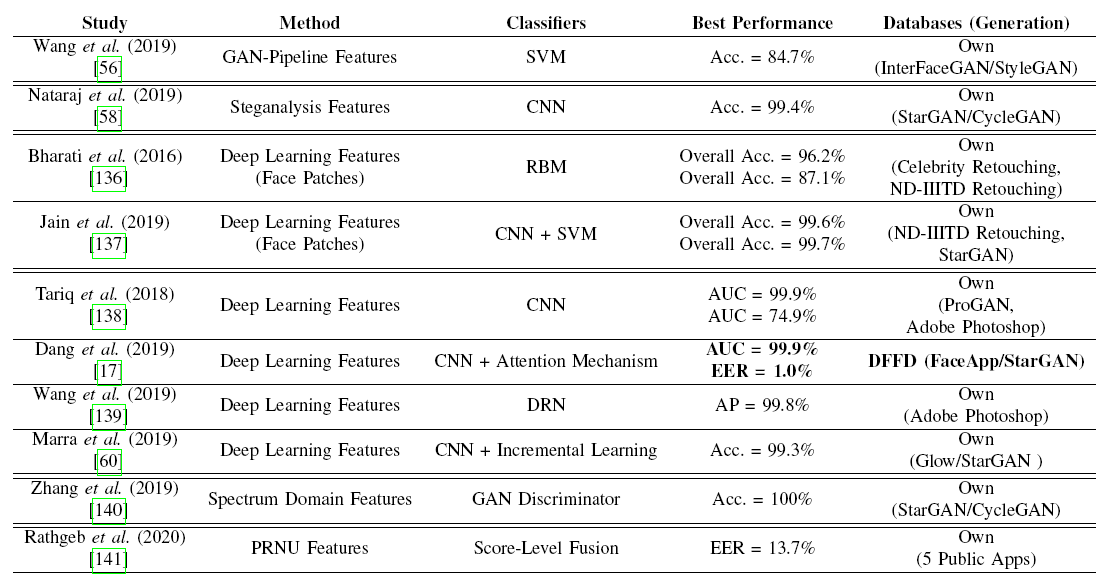
\includegraphics[width=\textwidth]{table-5-compare}
\label{table-5-compare}
\end{figure*}

Một số tác giả đề xuất phân tích pipeline GAN bên trong để phát hiện các artifact khác nhau giữa hình ảnh thực và hình ảnh được tổng hợp. Tương tự với các chỉnh sửa tổng hợp toàn bộ khuôn mặt, Wang và cộng sự đã dự đoán trong \Citet{wang1909fakespotter} rằng việc \textbf{giám sát hành vi của neuron cũng có thể đóng vai trò như một công cụ phát hiện} khuôn mặt giả vì các mẫu kích hoạt neuron từng lớp có thể nắm bắt các đặc điểm tinh tế quan trọng hơn. Phương pháp của họ được đặt tên là FakeSpoter, được trích xuất dưới dạng các đặc trưng bao phủ neuron của khuôn mặt thật và giả từ các hệ thống nhận dạng khuôn mặt sâu (VGG-Face \Citet{parkhi2015deep}, OpenFace \Citet{amos2016openface} và FaceNet \Citet{schroff2015facenet}), và sau đó huấn luyện một SVM cho phân loại cuối cùng. Các tác giả đã thử nghiệm phương pháp của họ bằng cách sử dụng các khuôn mặt thật từ cơ sở dữ liệu CelebA-HQ \Citet{karras2017progressive} và FFHQ \Citet{karras2019style} và các khuôn mặt tổng hợp được tạo thông qua InterFaceGAN \Citet{shen2020interpreting} và StyleGAN \Citet{karras2019style}, đạt được hiệu suất tốt nhất với độ chính xác phát hiện chỉnh sửa 84,7\% cuối cùng bằng cách sử dụng mô hình FaceNet.

Hệ thống phát hiện giả mạo \textbf{lấy cảm hứng từ phân tích mật mã} cũng đã được nghiên cứu. Như được mô tả trong \ref{sec:3-b-dectector} cho toàn bộ khuôn mặt, Nataraj và cộng sự đã đề xuất trong \Citet{nataraj2019detecting} một hệ thống phát hiện dựa trên sự kết hợp của ma trận đồng xuất hiện pixel và CNN. Họ đã tạo một tập dữ liệu giả mới dựa trên các chỉnh sửa thuộc tính bằng cách sử dụng phương pháp StarGAN \Citet{choi2018stargan} được huấn luyện thông qua cơ sở dữ liệu CelebA \Citet{liu2015deep}, đạt được độ chính xác tốt nhất 99,4\%.

Nhiều nghiên cứu cũng tập trung vào \textbf{các phương pháp học sâu thuần túy}, cung cấp cho mạng lưới các mảnh ghép mặt (face patches) hoặc với khuôn mặt hoàn chỉnh. Trong \Citep{bharati2016detecting}, Bharati và cộng sự đã đề xuất một phương pháp học sâu dựa trên Máy Boltzmann hạn chế (Restricted Boltzmann Machine - RBM) để phát hiện chỉnh sửa khuôn mặt. Đầu vào của hệ thống phát hiện bao gồm các mảnh ghép khuôn mặt để tìm hiểu các đặc trưng phân biệt để phân loại từng hình ảnh là ảnh gốc hoặc đã qua chỉnh sửa. Về cơ sở dữ liệu, các tác giả đã tạo ra hai cơ sở dữ liệu giả từ cơ sở dữ liệu ND-IIITD gốc (bộ sưu tập B \Citep{flynn2003assessment}) và một bộ ảnh khuôn mặt người nổi tiếng được tải xuống từ Internet. Hình ảnh giả được tạo ra bằng phần mềm chuyên nghiệp PortraitPro Studio Max24, xét đến các khía cạnh như kết cấu da, hình dạng của mắt, mũi, môi và tổng thể khuôn mặt, sự nổi bật của nụ cười, hình dạng môi và màu mắt… Cách tiếp cận đã đề xuất của họ đã đạt được độ chính xác tổng thể lần lượt là 96,2\% và 87,1\% đối với cơ sở dữ liệu chỉnh sửa người nổi tiếng và ND-IIITD.

Một cách tiếp cận tương tự \textbf{dựa trên các mảng mặt không chồng chéo} đã được trình bày trong \Citep{jain2018detecting}. Jain và cộng sự đã đề xuất một trình trích xuất đặc trưng CNN bao gồm 6 lớp phức hợp và 2 lớp được kết nối đầy đủ. Ngoài ra, các kết nối còn lại được coi là lấy cảm hứng từ kiến trúc ResNet. Cuối cùng, một SVM đã được sử dụng để phân loại cuối cùng. Về khung thử nghiệm, cơ sở dữ liệu chỉnh sửa ND-IIITD được trình bày đã được xem xét. Ngoài ra, các tác giả cho rằng hình ảnh giả được tạo ra thông qua cách tiếp cận StarGAN, được huấn luyện bằng cách sử dụng cơ sở dữ liệu CelebA. Nhìn chung, kết quả phát hiện tốt đạt được ở cả hai cách tiếp cận chỉnh sửa, đạt độ chính xác phát hiện chỉnh sửa gần như 100%.

\textbf{Phương pháp học sâu dựa trên mặt hoàn chỉnh} đã được nghiên cứu sâu hơn trong tài liệu, nhìn chung đạt được kết quả rất tốt. Tariq và cộng sự được đánh giá trong \Citep{tariq2018detecting} việc sử dụng các kiến trúc CNN khác nhau như VGG16, VGG19, ResNet, hoặc XceptionNet, trong số những kiến trúc khác. Đối với hình ảnh khuôn mặt thật, cơ sở dữ liệu CelebA đã được sử dụng. Về hình ảnh giả, hai cách tiếp cận khác nhau đã được xét: i) cách tiếp cận máy dựa trên GAN, cụ thể là ProGAN, và ii) cách tiếp cận thủ công dựa trên Adobe Photoshop CS6, bao gồm các chỉnh sửa như trang điểm, đeo kính, kính râm, tóc, và mũ nón. Để đánh giá thử nghiệm, các kích thước khác nhau của hình ảnh đã được xem xét (từ 32x32 đến 256x256 pixel). 99,99\% AUC đối với kịch bản do máy tạo ra, trong khi đối với kịch bản do con người tạo ra giá trị này giảm xuống còn 74,9\% AUC cho mô hình CNN tốt nhất. Do đó, hiệu suất phát hiện chỉnh sửa bị suy giảm cao đã được quan sát thấy giữa các hình ảnh giả do máy móc và con người tạo ra.

\textbf{Các cơ chế chú ý} cũng đã được áp dụng để cải thiện hơn nữa quá trình huấn luyện của các hệ thống phát hiện. Như đã mô tả trong các phần trước, Dang và cộng sự được phát triển một hệ thống có thể phát hiện các loại giả mạo khác nhau. Họ đã sử dụng cơ chế chú ý để xử lý và cải thiện bản đồ đặc trưng của các mô hình CNN. Về các chỉnh sửa thuộc tính, hai cách tiếp cận khác nhau đã được xét: i) hình ảnh giả được tạo thông qua phần mềm FaceApp công khai, với tối đa 28 bộ lọc khả dụng khác nhau xét các khía cạnh như tóc, tuổi, kính, râu và màu da, trong số những bộ lọc khác; và ii) hình ảnh giả được tạo ra thông qua cách tiếp cận StarGAN, với tối đa 40 bộ lọc khác nhau. Phương pháp tiếp cận đề xuất của họ đã được thử nghiệm bằng cách sử dụng cơ sở dữ liệu mới DFFD của họ, đạt được kết quả rất tốt gần 1,0% EER (và 99,9% AUC).

Wang và cộng sự được thực hiện trong \Citep{wang2019detecting} sử dụng phần mềm thương mại công khai từ Adobe Photoshop (công cụ Face-Aware Liquify) để tổng hợp các khuôn mặt mới, đồng thời cũng là một nghệ sĩ chuyên nghiệp để sáng tác 50 bức ảnh thật. Các tác giả bắt đầu thực hiện một nghiên cứu trên người thông qua Amazon Mechanical Turk (AMT), hiển thị hình ảnh thật và giả cho những người tham gia và yêu cầu họ phân loại từng hình ảnh vào một trong các lớp. Kết quả đạt được cho thấy độ khó của nhiệm vụ đối với con người, với độ chính xác cuối cùng là 53,5\%, gần như là may rủi (50\%). Sau khi nghiên cứu trên người, các tác giả đã đề xuất hai mô hình tự động khác nhau: i) mô hình phân loại toàn cầu dựa trên mạng dư lượng pha loãng (Dilated Residual Networks - DRN) để dự đoán xem khuôn mặt có bị cong vênh hay không, và ii) công cụ dự báo cong cục bộ dựa trên luồng quang học để xác định vị trí xảy ra chỉnh sửa và đảo ngược chúng. Phương pháp PWC-Net đã đề xuất trong \Citep{sun2018pwc} được coi là tính toán luồng từ ban đầu sang chỉnh sửa và ngược lại. Hiệu suất đạt 99,8\% và 97,4\% cho chỉnh sửa tổng hợp khuôn mặt tự động và thủ công.
Marra và cộng sự cũng được mô tả trong Sec. III-B có thể thực hiện phân biệt chính xác khi các GAN mới được đưa vào mạng và đạt được độ chính xác 99,3\%, dựa trên mô hình XceptionNet.

Zhang và cộng sự trong \Citep{zhang2019detecting} đưa ra một hình ảnh làm đầu vào, họ áp dụng DFT 2D cho mỗi kênh RGB, nhận được một hình ảnh tần số trên mỗi kênh. Về bộ phân loại, họ đề xuất AutoGAN, là một trình mô phỏng GAN có thể tổng hợp các tạo tác GAN trong bất kỳ hình ảnh nào mà không cần truy cập vào bất kỳ mô hình GAN nào được huấn luyện trước. Năng lực tổng quát hóa của phương pháp tiếp cận của họ đã được kiểm tra bằng cách sử dụng các mô hình GAN không nhìn thấy. Đặc biệt, StarGAN và GauGAN đã được xét trong đánh giá. Đối với phương pháp StarGAN, kết quả phát hiện tốt đã đạt được khi sử dụng miền tần số (100\%). Tuy nhiên, đối với phương pháp GauGAN, hiệu suất hệ thống bị suy giảm cao, độ chính xác 50\%. Các tác giả cho rằng điều này được tạo ra do bộ tạo của GauGAN khác hẳn với CycleGAN (được sử dụng trong huấn luyện).

Rathgeb và cộng sự đã đề xuất trong \Citep{rathgeb2020prnu} một hệ thống dựa trên sự không đồng nhất của phản hồi ảnh (PRNU). Cụ thể, điểm số thu được từ việc phân tích các đặc điểm không gian và quang phổ được trích xuất từ các mẫu PRNU trên các ô hình ảnh đã được hợp nhất. Cách tiếp cận đề xuất của họ được đánh giá trên cơ sở dữ liệu riêng tư được tạo bằng 5 ứng dụng di động khác nhau, đạt được EER trung bình 13,7\%.

Tóm lại, nhìn chung các phương pháp cung cấp kết quả rất tốt gần với độ chính xác 100\%, như được chỉ ra trong Bảng V. Điều này chủ yếu được tạo ra do thông tin dấu vân tay GAN hiện diện trong hình ảnh giả mạo. Tuy nhiên, như được chỉ ra trong toàn bộ chỉnh sửa tổng hợp khuôn mặt, các nghiên cứu gần đây đã đã đề xuất trong tài liệu để loại bỏ các dấu vân tay GAN như vậy khỏi ảnh giả trong khi vẫn giữ được vẻ ngoài rất thực tế, điều này thể hiện một thách thức ngay cả đối với những chương trình phát hiện chỉnh sửa tốt nhất.

\section{CHUYỂN ĐỔI BIỂU CẢM} \label{sec:6-expression}

\subsection{Kĩ thuật chỉnh sửa và Cơ sở dữ liệu công khai} \label{sec:6-a-technique}

Kĩ thuật này, còn được gọi là tái hiện khuôn mặt, bao gồm việc sửa đổi biểu hiện trên khuôn mặt của người đó. Các tác giả tập trung vào các kĩ thuật phổ biến nhất Face2Face và NeuralTextures, những kĩ thuật này thay thế nét mặt của một người trong video bằng nét mặt của người khác (trong video). Theo hiểu biết của nhóm tác giả, cơ sở dữ liệu hiện có duy nhất để nghiên cứu trong lĩnh vực này là FaceForensics ++.

Ban đầu, cơ sở dữ liệu FaceForensics tập trung vào phương pháp Face2Face. Đây là một phương pháp đồ họa máy tính chuyển biểu hiện của video nguồn sang video đích trong khi vẫn duy trì danh tính của người đích. Điều này được thực hiện thông qua lựa chọn khung hình chính thủ công. Cụ thể, các khung hình đầu tiên của mỗi video được sử dụng để nhận dạng khuôn mặt tạm thời (ví dụ mô hình 3D) và theo dõi biểu cảm trên các khung hình còn lại. Sau đó, các video giả được tạo bằng cách chuyển các tham số biểu cảm nguồn của mỗi khung hình (ví dụ 76 hệ số Blendshape) sang video đích. Sau đó, các tác giả đã trình bày trong FaceForensics ++ một cách tiếp cận học tập mới dựa trên NeuralTextures. Đây là một phương pháp output sử dụng dữ liệu video gốc để tìm hiểu cấu trúc mạng neuron của người mục tiêu, bao gồm cả mạng output. Đặc biệt, các tác giả đã xem xét trong quá trình triển khai của họ một sự mất mát GAN dựa trên từng phần mặt như được sử dụng trong Pix2Pix. Chỉ có nét mặt tương ứng với miệng được sửa đổi. Điều quan trọng cần lưu ý là tất cả dữ liệu đều có sẵn trên FaceForensics ++ trên GitHub. Tổng cộng có 1.000 video thực được trích xuất từ Youtube. Đối với các video bị giả, có 2.000 video giả mạo (1.000 video cho mỗi cách tiếp cận được coi là giả mạo). Ngoài ra, cần nhấn mạnh rằng các mức chất lượng video khác nhau đã được xét, cụ thể: i) RAW (chất lượng gốc), ii) HQ (tần số lấy mẫu 23) và iii) LQ (tần số lấy mẫu 40). Cách lấy mẫu này mô phỏng các kĩ thuật xử lý video thường được áp dụng trong mạng xã hội.

Ngoài các kĩ thuật Face2Face và NeuralTexture được xét trong các chỉnh sửa hoán đổi biểu cảm ở cấp độ video, các phương pháp tiếp cận khác nhau gần đây đã đề xuất để thay đổi biểu cảm khuôn mặt trong cả hình ảnh và video. Một cách tiếp cận rất phổ biến đã được trình bày trong \Citep{averbuch2017bringing}. Averbuch-Elor và cộng sự đã đề xuất một kĩ thuật để tự động tạo hoạt ảnh cho một bức chân dung tĩnh bằng cách sử dụng video của một chủ thể khác, chuyển sự biểu cảm của chủ thể video sang chân dung mục tiêu. Không giống như các phương pháp tiếp cận Face2Face và NeuralTexture yêu cầu video từ cả khuôn mặt đầu vào và khuôn mặt mục tiêu, chỉ cần một hình ảnh của mục tiêu. Trong nhánh này, một phương pháp gần đây đã được trình bày trong \Citep{zakharov2019few}, mang lại kết quả rất tốt trong cả việc học một lần (one shot learning) và ít lần (few shots learning).

Cuối cùng, nhóm tác giả cũng nêu bật các cách tiếp cận phổ biến khác ở cấp độ hình ảnh. Ví dụ, các ứng dụng di động như FaceApp cho phép dễ dàng thay đổi mức độ cười, từ vui vẻ sang tức giận hơn. Các cách tiếp cận này dựa trên kiến trúc GAN hiện tại. Ví dụ, Choi và cộng sự \Citet{choi2018stargan} cho thấy tiềm năng của StarGAN trong việc thay đổi hình ảnh đầu vào sang các mức độ biểu hiện khác nhau như tức giận, vui vẻ, trung tính, buồn bã, ngạc nhiên và sợ hãi. Các phương pháp GAN gần đây khác giúp cải thiện cả chất lượng hình ảnh của ảnh giả và việc chỉnh sửa điều khiển các thông số là InterFaceGAN, UGAN, STGAN và AttGAN.

\subsection{Phát hiện chỉnh sửa} \label{sec:6-b-detector}

Phần này nhằm mục đích cung cấp tổng quan về công cụ phát hiện hoán đổi biểu cảm ở cấp độ video bằng cách sử dụng cơ sở dữ liệu FaceForensics ++, vì đây là cơ sở dữ liệu công khai duy nhất dành cho nghiên cứu trong lĩnh vực này, theo hiểu biết của nhóm tác giả. Các chỉnh sửa ở cấp độ hình ảnh (không phải video) có thể được phát hiện bằng cách sử dụng các phương pháp tương tự được mô tả trong Phần. III-B và V-B.

Bảng VI cung cấp so sánh các phương pháp tiếp cận phù hợp nhất trong lĩnh vực phát hiện hoán đổi biểu cảm. Đối với mỗi nghiên cứu, nhóm tác giả bao gồm thông tin liên quan đến phương pháp, bộ phân loại, hiệu suất tốt nhất và cơ sở dữ liệu. Các tác giả nhấn mạnh kết quả tốt nhất đạt được cho cơ sở dữ liệu công khai duy nhất, FaceForensics ++. Điều quan trọng cần lưu ý là trong một số trường hợp, các số liệu được đánh giá khác nhau được xét gây khó khăn cho việc so sánh công bằng giữa các nghiên cứu.


\begin{figure*}[h!]
\caption{Bảng VI: So sánh các cách phát hiện}
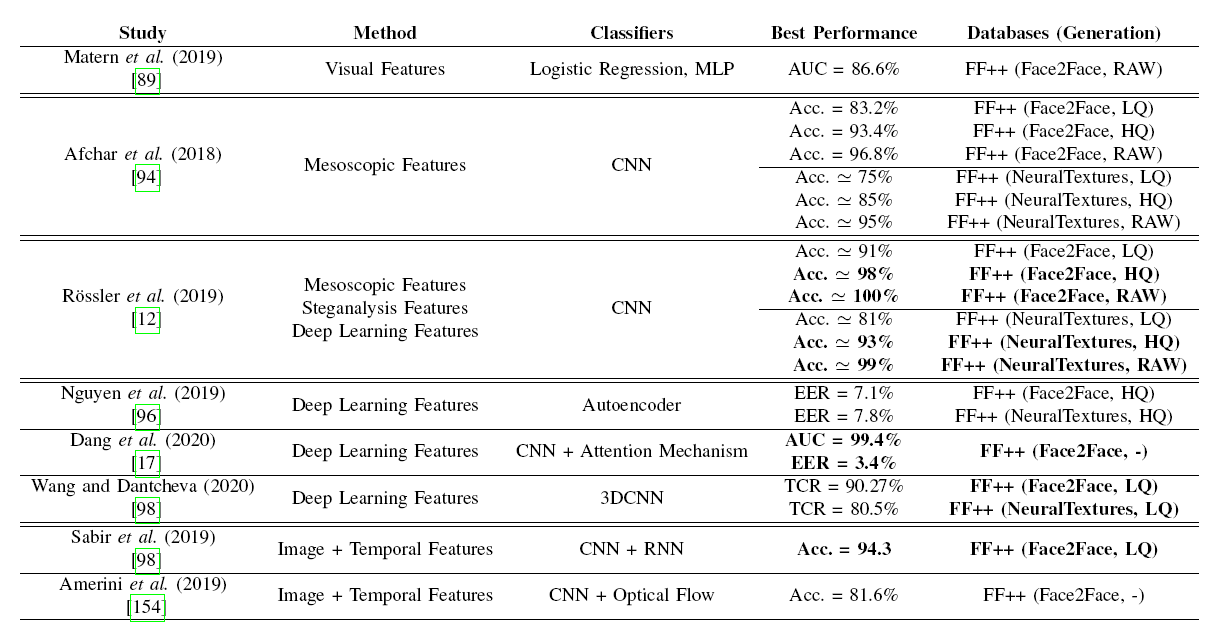
\includegraphics[width=\textwidth]{table-6-compare}
\label{table-6-compare}
\end{figure*}

Một số phương pháp sau đây đã được thảo luận trong \ref{sec:4-b-detector} để hoán đổi danh tính. Sau đây nhóm tác giả tóm tắt kết quả họ đạt được trong việc phát hiện các chỉnh sửa hoán đổi biểu cảm.

Các nghiên cứu sơ bộ đã tập trung vào các đặc điểm hình ảnh tồn tại trong video giả như màu mắt, phản xạ bị thiếu, … Matern và cộng sự, phương pháp được thử nghiệm bằng FaceForensics ++, chỉ có kĩ thuật chỉnh sửa Face2Face, đạt được kết quả cuối cùng 86,6% AUC.

Các phương pháp tiếp cận dựa trên các đặc điểm của kính trung mô và phân tích ẩn cũng đã được nghiên cứu trong tài liệu. Trong \Citet{afchar2018mesonet}, cách tiếp cận đã đề xuất đã được thử nghiệm bằng cách sử dụng video giả Face2Face từ cơ sở dữ liệu FaceForensics ++, đạt được kết quả nói chung là tốt, đặc biệt là đối với video chất lượng RAW. Phương pháp tương tự sau đó đã được thử nghiệm chống lại các video giả mạo NeuralTextures, thu được kết quả có độ chính xác thấp hơn so với Face2Face.

Phương pháp học sâu gần đây cũng được áp dụng với kết quả tốt. Trong \Citet{cite12}, hệ thống phát hiện dựa trên XceptionNet đã cung cấp kết quả tốt nhất trong cả chỉnh sửa Face2Face và NeuralTextures, gần 100\% với chất lượng RAW. Ngoài ra, các hệ thống phát hiện đã được đánh giá xem xét các mức chất lượng video khác nhau để mô phỏng quá trình xử lý video của nhiều mạng xã hội. Trong tình huống thực tế này, độ chính xác của tất cả các hệ thống phát hiện đã bị giảm chất lượng như nó xảy ra trong các chỉnh sửa hoán đổi danh tính.

Trong \Citet{nguyen2019multi}, cách tiếp cận đã đề xuất dựa trên việc học đa tác vụ đã được đánh giá với cơ sở dữ liệu FaceForensics ++. Đối với phương pháp Face2Face, EER 7,1\% đã đạt được trên video HQ trong khi đối với phương pháp NeuralTexture, EER đã tăng thêm một chút lên mức EER 7,8\% cuối cùng khi phát hiện chỉnh sửa.

Các cơ chế chú ý gần đây đã đã đề xuất trong \Citet{dang2020detection} để cải thiện thêm quá trình huấn luyện. Phương pháp phát hiện đã đề xuất đã được thử nghiệm bằng cách sử dụng cơ sở dữ liệu DFFD, cho chỉnh sửa hoán đổi biểu cảm chỉ dựa trên dữ liệu từ cơ sở dữ liệu FaceForensics ++. Phương pháp đề xuất đạt được AUC = 99,4\% và EER = 3,4\%.

Các phương pháp tiếp cận học sâu dựa trên 3DCNN đã được nghiên cứu trong \Citep{wang2020video} để xem xét cả thông tin không gian và chuyển động. Tương tự như chỉnh sửa hoán đổi danh tính, các tác giả đề xuất bộ phát hiện giả mạo dựa trên phương pháp tiếp cận I3D và 3D ResNet, đạt được kết quả hứa hẹn trên các video chất lượng thấp của cơ sở dữ liệu FaceForensics ++.

\textbf{Dựa trên việc phân tích cả hình ảnh và thông tin thời gian}. Trong \Citet{sabir2019recurrent}, phương pháp tiếp cận đã đề xuất dựa trên mạng tích chập lặp lại đã được thử nghiệm bằng cách sử dụng cơ sở dữ liệu FaceForensics ++, đạt được kết quả AUC là 94,3\% đối với kĩ thuật Face2Face. Chỉ những video chất lượng thấp mới được xét trong phân tích. Cuối cùng, trong \Citep{amerini2019deepfake}, Amerini và cộng sự đề xuất áp dụng trường luồng quang để khai thác sự khác biệt giữa các khung hình có thể có, sử dụng phương pháp PWC-Net \Citep{sun2018pwc}. Luồng quang học là một trường vectơ được tính toán giữa các khung hình liên tiếp để trích xuất chuyển động biểu kiến trong cảnh. Việc sử dụng phương pháp này được thúc đẩy vì video giả sẽ có luồng quang học không tự nhiên do chuyển động bất thường của môi, mắt, … Kết quả ban đầu thu được bằng cách sử dụng cả hai mạng VGG16 và ResNet50, đạt được ACC 81,6%.

Như đã nêu trên, hầu hết các phương pháp được báo cáo ở đây để phát hiện hoán đổi biểu cảm cũng đã được sử dụng để phát hiện hoán đổi danh tính như đã xem xét trong Phần. IV-B. Nói chung, có vẻ như các đặc trưng tương tự có thể được học bởi bộ phát hiện giả để phân biệt giữa nội dung thật và giả, đạt được kết quả tốt trong cả hai loại chỉnh sửa.

\section{NHỮNG HƯỚNG CHỈNH SỬA KHUÔN MẶT KHÁC} \label{sec:7-other-direction}

Bốn lớp kĩ thuật chỉnh sửa trên khuôn mặt được mô tả trước đây là những kĩ thuật đang nhận được nhiều sự chú ý nhất trong vài năm qua, nhưng chúng không đại diện hoàn hảo cho tất cả các chỉnh sửa có thể có trên khuôn mặt. Phần này thảo luận về một số cách tiếp cận đầy thách thức và nguy hiểm khác trong chỉnh sửa trên khuôn mặt: biến hình khuôn mặt, nhận dạng khuôn mặt và tổng hợp khuôn mặt dựa trên âm thanh hoặc văn bản (ví dụ âm thanh thành video và văn bản thành video).

\subsection{Biến hình khuôn mặt} \label{sec:7-a-face-mophism}

Biến hình khuôn mặt là một loại chỉnh sửa trên khuôn mặt có thể được sử dụng để tạo ra các mẫu khuôn mặt sinh trắc nhân tạo giống với thông tin sinh trắc học của hai hoặc nhiều cá thể \Citep{wolberg1998image}, \Citep{scherhag2019face}. Điều này có nghĩa là hình ảnh khuôn mặt được biến đổi mới sẽ được xác minh thành công dựa trên các mẫu khuôn mặt của hai hoặc nhiều cá nhân, tạo ra mối đe dọa nghiêm trọng đối với hệ thống nhận dạng khuôn mặt \Citep{gomez2017your}, \Citep{korshunov2019vulnerability}. Theo nghĩa này, biến hình khuôn mặt là một kiểu chỉnh sửa trên khuôn mặt khác với bốn kiểu chính được đề cập trong bài báo này. Cần lưu ý rằng biến đổi khuôn mặt chủ yếu tập trung vào việc tạo ra các mẫu giả ở cấp độ hình ảnh, chứ không phải video như các chỉnh sửa hoán đổi danh tính.

Gần đây đã có một lượng lớn các nghiên cứu trong lĩnh vực biến hình khuôn mặt. Một đánh giá rất đầy đủ về lĩnh vực này đã được đăng bởi Scherhag và cộng sự \Citep{scherhag2019face} vào năm 2019 bao gồm cả kĩ thuật biến hình và cả công cụ phát hiện tấn công biến hình. Mặc dù có số lượng công bố lớn, nhưng nghiên cứu trong lĩnh vực này vẫn còn sơ khai, còn nhiều vấn đề và thách thức còn bỏ ngỏ. Điều quan trọng là phải làm nổi bật việc thiếu các cơ sở dữ liệu công khai và các tiêu chuẩn đánh giá điều này gây khó khăn cho việc so sánh công bằng giữa các nghiên cứu. Để khắc phục khía cạnh này, Raja và cộng sự gần đây đã trình bày một khuôn khổ thú vị để phát hiện tấn công biến hình \Citep{raja2020morphing}, bao gồm cơ sở dữ liệu công khai, nền tảng đánh giá và điểm chuẩn. Cơ sở dữ liệu bao gồm các hình ảnh thực và ảo tạo thành 1.800 bức ảnh của 150 đối tượng. Hình ảnh biến đổi được tạo ra bằng cách sử dụng 6 thuật toán khác nhau, đưa ra nhiều cách tiếp cận khả thi.

Liên quan đến chương trình phát hiện khuôn mặt bị sửa, các phương pháp tiếp cận khác nhau đã đề xuất trong tài liệu dựa trên các đặc điểm khác nhau, ví dụ: giảm chi tiết khuôn mặt do hoạt động trộn \Citep{kraetzer2017modeling}, phổ Fourier của nhiễu mẫu cảm biến \Citep{zhang2018face}, sự khác biệt giữa các điểm mốc trên khuôn mặt \Citep{scherhag2018detecting}, \Citep{damer2018detecting}, và các đặc trưng học sâu thuần túy \Citep{ferrara2019face}, \Citep{scherhag2020deep}. Ngoài ra, các phương pháp tiếp cận dựa trên biến hình khuôn mặt đã được nghiên cứu để khôi phục hình ảnh khuôn mặt của đồng phạm \Citep{ferrara2017face}, \Citep{peng2019fd}.

\subsection{Khử nhận dạng khuôn mặt} \label{sec:7-b-de-id}

Mục tiêu chính của việc khử nhận dạng khuôn mặt (de-ID) là loại bỏ thông tin nhận dạng có trên hình ảnh hoặc video khuôn mặt để bảo vệ quyền riêng tư của người đó \Citep{gross2006model}. Điều này có thể đạt được bằng một số cách. Cách đơn giản nhất có thể là làm mờ khuôn mặt bằng cách làm mờ hoặc tạo pixel (ví dụ: trong Chế độ xem phố của Google Maps). Các phương pháp phức tạp hơn cố gắng cung cấp hình ảnh khuôn mặt với các đặc điểm nhận dạng khác nhau nhưng vẫn duy trì tất cả các yếu tố khác (tư thế, biểu cảm, ánh sáng, …) không thay đổi. Do đó, khái niệm về khuôn mặt de-ID là rất chung chung. Một lựa chọn khả thi có thể là thông qua hoán đổi nhận dạng khuôn mặt.

Các công trình trước đây trong lĩnh vực này dựa trên việc áp dụng deID khuôn mặt cho ảnh tĩnh. Trong \Citep{gross2009face} Gross và cộng sự đã trình bày một khung đa yếu tố cho de-ID, kết hợp các mô hình tuyến tính, song tuyến và bậc hai. Họ cho thấy phương pháp của họ có thể bảo vệ quyền riêng tư trong khi vẫn bảo toàn tiện ích dữ liệu trên cơ sở dữ liệu khuôn mặt biểu hiện. Gần đây, sự phát triển của các phương pháp tổng hợp hình ảnh dựa trên mạng neuron sâu sinh sản, đặc biệt là GAN, đã truyền cảm hứng cho các phương pháp khử ID khuôn mặt mới như \Citep{meden2017face} - \Citep{pan2019k}, sử dụng các khuôn mặt tổng hợp để thay thế các khuôn mặt ban đầu. Ngoài ra, trong \Citep{mirjalili2019flowsan}, các tác giả đã đề xuất việc sử dụng Mạng bán đối thủ (SAN) để làm nhiễu các bộ phân loại giới tính dựa trên khuôn mặt tùy ý.

Gần đây hơn, trong \Citep{gafni2019live} Gafni và cộng sự giới thiệu vào năm 2019, một phương pháp cung cấp đặc trưng khử ID bằng khuôn mặt với hiệu suất thuyết phục ngay cả trong các video không bị giới hạn. Cách tiếp cận của họ dựa trên một bộ autoencoder đối nghịch kết hợp với một bộ phân loại khuôn mặt được huấn luyện. Bằng cách này, họ có thể đạt được không gian tiềm ẩn phong phú, nhúng cả thông tin nhận dạng và biểu hiện. Ngoài ra, trong \Citep{li2019identification} một phương pháp khử ID khuôn mặt mới dựa trên mô hình chuyển sâu đã được trình bày. Phương pháp này coi các thuộc tính khuôn mặt không liên quan đến danh tính như kiểu dáng của khuôn mặt ban đầu và sử dụng mô hình chuyển thuộc tính khuôn mặt được huấn luyện để trích xuất và ánh xạ chúng với các khuôn mặt khác nhau, đạt được kết quả rất hứa hẹn cả về hình ảnh và video.

Một số nghiên cứu liên quan khác trong lĩnh vực này làm việc trực tiếp trên các biểu diễn khuôn mặt hoặc mô hình khuôn mặt sâu bằng cách loại bỏ ở đó những thông tin không mong muốn hoặc được bảo vệ như danh tính, giới tính hoặc nét mặt \Citep{alvi2018turning} - \Citep{gong2019debface}. Sau khi thông tin được bảo vệ đó đã bị loại bỏ, một hình ảnh khuôn mặt hoặc video sau đó có thể được tạo dựa trên các hình ảnh đại diện mới có nguồn gốc trong đó thông tin được bảo vệ đã bị loại bỏ, giảm bớt hoặc làm xáo trộn.

\subsection{Audio-to-Video and Text-to-Video} \label{sec:7-c-atov-ttov}

Một chủ đề liên quan đến hoán đổi nét mặt là tổng hợp video từ âm thanh hoặc văn bản. Những kiểu chỉnh sửa trên khuôn mặt bằng video này còn được gọi là trò giả mạo lip-sync \Citep{agarwal2020detecting}. Các ví dụ phổ biến có thể được tìm thấy trên Internet.

Về việc tổng hợp video giả từ âm thanh (audio-to-video), Suwajanakorn và cộng sự được trình bày trong \Citep{suwajanakorn2017synthesizing} phương pháp tổng hợp video chất lượng cao về một người (trong trường hợp này là Obama) nói nhép chính xác. Họ đã sử dụng làm đầu vào cho phương pháp tiếp cận các video trước đó của họ trong nhiều giờ về người đó cùng với bản ghi âm mới. Trong cách tiếp cận của mình, họ đã sử dụng một mạng neuron lặp lại (dựa trên LSTM) để học cách ánh xạ từ các đặc điểm âm thanh thô đến hình dạng miệng. Sau đó, dựa trên hình dạng miệng ở mỗi khung hình, họ tổng hợp kết cấu miệng chất lượng cao và kết hợp nó với khớp tư thế 3D để tạo ra video mới khớp với bản âm thanh đầu vào, tạo ra kết quả chân thực.

Trong \Citep{song2018talking}, Song và cộng sự đã đề xuất một cách tiếp cận dựa trên một mạng tạo lặp lại có điều kiện mới (conditional recurrent generation network), kết hợp cả các đặc trưng hình ảnh và âm thanh trong đơn vị lặp lại để phụ thuộc theo thời gian và cũng có một cặp phân biệt không gian-thời gian để có chất lượng hình ảnh / video tốt hơn. Do đó, cách tiếp cận của họ có thể mô hình hóa cả môi và miệng cùng với các biến thể biểu cảm và tư thế đầu nói chung, đạt được kết quả thực tế hơn nhiều. Mã nguồn được công bố công khai trong GitHub, ngoài ra, trong \Citep{song2020everybody} Song và cộng sự đã trình bày một phương pháp động không giả định một mạng kết xuất dành riêng cho từng người. Trong cách tiếp cận của mình, họ có thể tạo video giả rất thực tế bằng cách thực hiện tái tạo mô hình khuôn mặt 3D từ video đầu vào cộng với mạng lặp lại để chuyển âm thanh nguồn thành các thông số biểu hiện. Cuối cùng, họ đã giới thiệu một mạng kết xuất video mới lạ và một phương pháp lập trình động để tạo ra một video giống như hình ảnh và mạch lạc nhất thời. Kết quả video được hiển thị trên Internet. Một cách tiếp cận thú vị khác đã được trình bày trong \Citep{zhou2019talking} Zhou và cộng sự đã đề xuất một khung mới có tên là Disentangled AudioVisual System (DAVS), tạo ra các video khuôn mặt nói chuyện chất lượng cao bằng cách sử dụng biểu diễn âm thanh-hình ảnh không tách rời. Cả thông tin giọng nói âm thanh và video đều có thể được sử dụng làm hướng dẫn đầu vào. Mã nguồn có sẵn trên GitHub.

Về việc tổng hợp video giả từ văn bản (text-to-video), Fried và cộng sự đã đề xuất trong \Citep{fried2019text} một phương pháp lấy đầu vào là video của một người đang nói và văn bản mong muốn được nói, đồng thời tổng hợp một video mới trong đó miệng của người đó được đồng bộ hóa với các từ mới. Đặc biệt, phương pháp của họ tự động chú thích một video đầu vào với âm vị, hình ảnh, tư thế khuôn mặt và hình học 3D, độ phản chiếu, biểu cảm và độ sáng cảnh trên mỗi khung hình. Cuối cùng, một mạng recurrent video generation network tạo ra một video chân thực khớp với bản ghi đã chỉnh sửa. Ví dụ về các video giả mạo được tạo bằng cách tiếp cận này được công bố công khai.

Theo hiểu biết của nhóm tác giả, không có cơ sở dữ liệu và tiêu chuẩn công khai nào liên quan đến nội dung phát hiện giả mạo âm thanh và văn bản thành video. Nghiên cứu về chủ đề này thường được thực hiện thông qua việc tổng hợp dữ liệu nội bộ bằng cách sử dụng các mã nguồn có sẵn công khai như những mã nguồn được giới trong phần này.

Các nghiên cứu gần đây đã phân tích mức độ dễ dàng phát hiện nội dung giả mạo âm thanh và văn bản thành video. Trong \Citep{agarwal2020detecting}, Agarwal và cộng sự đã đề xuất một phương pháp phát hiện giả nhằm khai thác sự mâu thuẫn tồn tại giữa động lực của hình dạng miệng (visemes) và âm vị nói. Họ tập trung vào một số cảnh cụ thể trong đó miệng phải được đóng lại hoàn toàn và nhận thấy rằng điều này đã không xảy ra trong nhiều video bị sửa. Cách tiếp cận của họ đã đạt được kết quả tốt, đặc biệt khi thời lượng của video tăng lên.

\section{KÊT LUẬN} \label{sec:8-conclusion}

Bài báo này này cung cấp bức tranh toàn cảnh về lĩnh vực chỉnh sửa kĩ thuật số trên khuôn mặt, bao gồm các chi tiết cập nhật: i) các loại chỉnh sửa trên khuôn mặt, ii) các kĩ thuật chỉnh sửa trên khuôn mặt, iii) cơ sở dữ liệu công khai cho nghiên cứu, và iv) các tiêu chuẩn để phát hiện từng nhóm chỉnh sửa trên khuôn mặt, bao gồm các kết quả chính đạt được bằng các phương pháp tiếp cận phát hiện chỉnh sửa tiêu biểu nhất.

Nói chung, hầu hết các chỉnh sửa trên khuôn mặt hiện tại dường như dễ bị phát hiện trong các tình huống được kiểm soát, ví dụ khi các máy phát hiện giả được đánh giá trong cùng điều kiện mà chúng được huấn luyện. Thực tế này đã được chứng minh trong hầu hết các điểm chuẩn được đưa vào bài báo này, đạt tỷ lệ lỗi rất thấp trong việc phát hiện chỉnh sửa. Tuy nhiên, viễn cảnh này có thể không thực tế lắm vì các hình ảnh và video giả thường được chia sẻ trên mạng xã hội, có nhiều biến thể như mức độ nén, thay đổi kích thước, độ nhiễu, … Ngoài ra, các kĩ thuật chỉnh sửa trên khuôn mặt cũng không ngừng được cải thiện. Những yếu tố này thúc đẩy các nghiên cứu sâu hơn về khả năng tổng quát hóa của các chương trình phát hiện giả trong điều kiện chưa từng quan sát. Nghiên cứu trong tương lai có thể dựa trên các nghiên cứu mới nhất vì chúng không yêu cầu các video giả để huấn luyện, cung cấp khả năng tổng quát hóa tốt hơn để chống lại các cuộc tấn công với dữ liệu chưa từng huấn luyện.

Các kĩ thuật kết hợp, ở cấp độ đặc trưng hoặc điểm số, có thể cung cấp sự linh hoạt hơn của các chương trình giả với các tình huống khác nhau. Trên thực tế, các phương pháp phát hiện giả mạo khác nhau đã dựa trên sự kết hợp của các nguồn thông tin khác nhau, ví dụ, Zhou và cộng sự đề xuất trong \Citet{zhou2017two} một hệ thống phát hiện dựa trên sự kết hợp của phân tích ẩn và các đặc trưng học sâu thuần túy, trong khi Rathgeb và cộng sự đề xuất trong \Citep{rathgeb2020prnu} sự kết hợp của các đặc trưng không gian và quang phổ. Hai cách tiếp cận tổng hợp thú vị khác gần đây đã được trình bày trong \Citep{yang2020pipenet}, \Citep{yu2020multi}, kết hợp thông tin RGB, độ sâu và hồng ngoại để phát hiện các cuộc tấn công khuôn mặt vật lý. Ngoài ra, các phương pháp tiếp cận trọng số khuôn mặt đã đã đề xuất để phát hiện video giả sử dụng nhiều khung hình \Citep{montserrat2020deepfakes}. Cuối cùng, việc tổng hợp các nguồn thông tin khác như văn bản, cách gõ phím hoặc âm thanh đi kèm với video khi tải chúng lên mạng xã hội có thể rất có giá trị để cải thiện trình phát hiện \Citep{agrawal2017multimodal} - \Citep{morales2020keystroke}.

Ngoài các công cụ phát hiện giả truyền thống chỉ dựa trên thông tin hình ảnh / video, các phương án mới nên được nghiên cứu để cung cấp các công cụ mạnh mẽ hơn. Một ví dụ về điều này là công trình được trình bày bởi Tursman và cộng sự trong \Citep{tursman2020towards}. Các tác giả đề xuất phát hiện nội dung giả mạo thông qua xác minh trên mạng xã hội tại thời điểm nắm bắt: trọng tài xác minh tính trung thực là một nhóm máy quay video chụp đồng bộ một người nói, đạt được sự đồng thuận chung, sau đó ký tên vào video của họ trong thời gian thực là “thật”. Các cách tiếp cận như thế này có thể bảo vệ nội dung phương tiện khỏi các cuộc tấn công hơn nữa.

Tiếp theo, nhóm tác giả nêu bật các khía cạnh chính cần cải thiện và các xu hướng trong tương lai cần tuân theo cho từng nhóm chỉnh sửa trên khuôn mặt:

\textbf{Tổng hợp khuôn mặt}: các chỉnh sửa hiện nay thường dựa trên kiến trúc GAN như StyleGAN, cung cấp hình ảnh rất chân thực. Tuy nhiên, hầu hết các chương trình có thể dễ dàng phân biệt giữa hình ảnh thật và giả, đạt được độ chính xác gần 100\%. Điều này được tạo ra do hình ảnh giả được đặc trưng bởi các dấu vân tay GAN cụ thể. Nhưng, điều gì sẽ xảy ra nếu chúng ta có thể loại bỏ các dấu vân tay GAN đó hoặc thêm một số mẫu nhiễu trong khi vẫn giữ được những hình ảnh tổng hợp rất chân thực? Các phương pháp tiếp cận gần đây tập trung vào dòng nghiên cứu này, điều này thể hiện một thách thức ngay cả đối với các hệ thống phát hiện chỉnh sửa tốt nhất.

\textbf{Hoán đổi danh tính}: mặc dù nhiều cách tiếp cận khác nhau đã đã đề xuất trong tài liệu, nhưng chắc chắn rất khó để quyết định cách nào là tốt nhất. Đầu tiên, hầu hết các cách tiếp cận đều được huấn luyện cho một cơ sở dữ liệu và mức nén cụ thể, nói chung đạt được kết quả rất tốt. Tuy nhiên, tất cả chúng đều cho kết quả tổng quát hóa kém đối với các điều kiện chưa từng được gặp. Ngoài ra, thực tế là các số liệu khác nhau (ví dụ: Acc., AUC, EER, …) và các giao thức thử nghiệm thường được coi là không giúp đạt được sự so sánh công bằng giữa các nghiên cứu. Tất cả những khía cạnh này cần được xem xét thêm để phát triển trong lĩnh vực này.

Hơn nữa, nhóm tác giả muốn làm nổi bật kết quả phát hiện đạt được trong cơ sở dữ liệu DeepFake mới nhất của thế hệ thứ 2 như DFDC và Celeb-DF. Mặc dù các máy phát hiện giả đã đạt được kết quả AUC gần 100\% trong cơ sở dữ liệu thế hệ 1 như UADFV và FaceForensics ++, chúng đều bị suy giảm hiệu suất cao trên những cái mới nhất, đặc biệt là đối với Celeb-DF cơ sở dữ liệu với kết quả AUC dưới 60\% trong hầu hết các trường hợp. Do đó, cần nhiều nỗ lực hơn nữa để cải thiện hơn nữa các hệ thống phát hiện giả mạo hiện tại, chẳng hạn như thông qua các thử thách và điểm chuẩn quy mô lớn như DFDC34 gần đây.

\textbf{Kĩ thuật thuộc tính}: cùng một khía cạnh được đánh dấu cho tổng hợp khuôn mặt (loại bỏ dấu vân tay GAN) cũng được áp dụng ở đây vì hầu hết các chỉnh sửa đều dựa trên kiến trúc GAN. Ngoài ra, cũng rất thú vị khi nhận xét sự khan hiếm của cơ sở dữ liệu công khai cho nghiên cứu (chỉ có cơ sở dữ liệu DFFD được công bố công khai) và thiếu các giao thức thử nghiệm tiêu chuẩn để thực hiện so sánh công bằng giữa các nghiên cứu.

\textbf{Hoán đổi biểu cảm}: trái với hoán đổi danh tính, đã phát triển nhanh chóng với việc các cơ sở dữ liệu DeepFake cải tiến được phát hành, cơ sở dữ liệu công khai duy nhất trong hoán đổi biểu cảm là FaceForensics ++, theo hiểu biết của nhóm tác giả. Cơ sở dữ liệu này được đặc trưng bởi các hiện vật trực quan dễ phát hiện, do đó, kết quả AUC đạt được gần 100\% trong một số phương pháp phát hiện giả mạo. Các tác giả khuyến khích các nhà nghiên cứu tạo và công khai các cơ sở dữ liệu thực tế hơn dựa trên các kĩ thuật gần đây.

Tất cả những khía cạnh này, cùng với sự phát triển của các phương pháp tiếp cận GAN cải tiến và Thách thức phát hiện DeepFake (DFDC) gần đây sẽ thúc đẩy thế hệ hình ảnh / video giả thực tế mới cùng với các kĩ thuật tiên tiến hơn để phát hiện chỉnh sửa trên khuôn mặt.



\bibliographystyle{acl_natbib}
\bibliography{custom}

\end{document}
